\documentclass[12pt,a4paper,oneside]{report}

%-------------------- Page layout and fonts --------------------------
\usepackage[a4paper,left=1.25in,right=1in,top=1in,bottom=1in,headheight=15pt]{geometry}
% Font: LaTeX default Computer Modern (cmr) throughout --- do not load other font packages
\usepackage{eso-pic}             % page border on front-matter pages
\usepackage{setspace}
\onehalfspacing
\usepackage{microtype}

%-------------------- Packages ---------------------------------------
\usepackage{graphicx}
\usepackage{amsmath,amssymb}
\usepackage{booktabs,tabularx,multirow,longtable,array}
\usepackage{float}
\usepackage[font=small,labelfont=bf]{caption}
\usepackage{enumitem}
\usepackage[dvipsnames,table]{xcolor}
\usepackage{tikz}
\usetikzlibrary{arrows.meta,positioning,shapes.geometric,fit,backgrounds}
\usepackage{pgfplots}
\pgfplotsset{compat=1.17}
\usepackage{algorithm}
\usepackage{algpseudocode}
\usepackage{listings}
\usepackage[most]{tcolorbox}
\usepackage{fancyhdr}
\usepackage{titlesec}
\usepackage{hyperref}
\hypersetup{
    bookmarksopen=true,
    colorlinks=true,
    citecolor=blue,
    linkcolor=blue,
    urlcolor=blue
}

%=====================================================================
%  PROJECT DETAILS --- EDIT THIS BLOCK
%=====================================================================
\newcommand{\ProjectTitle}{ReCycleGuard: An Agentic Assistant for Auditable E-Waste EPR Compliance Reconciliation}
% Short title for the page header (shorten if it does not fit on one line)
\newcommand{\HeaderTitle}{ReCycleGuard: Agentic E-Waste EPR Reconciliation}
\newcommand{\TeamNo}{\pendingtext{team number}}
\newcommand{\AcademicYear}{2026--27}
\newcommand{\SubmissionDate}{12 November 2026}
% Team members: USN and Name (delete the 4th row in the tables if you have only 3 members)
\newcommand{\USNa}{1BM23CD020}  \newcommand{\NameA}{H Sampreeth Bhat}
\newcommand{\USNb}{1BM23CD047}  \newcommand{\NameB}{R V Abhishek}
\newcommand{\USNc}{1BM23CD063}  \newcommand{\NameC}{Sushanth S}
\newcommand{\USNd}{1BM23CD069}  \newcommand{\NameD}{Vedantha Vinay Vernekar}
% Course lead
\newcommand{\GuideName}{Dr. Kalyan Nagaraj}
\newcommand{\GuideDesig}{Assistant Professor}

%=====================================================================
%  GUIDANCE SWITCH: set to \guidancefalse before final submission
%=====================================================================
\newif\ifguidance
\guidancefalse

%-------------------- Colours and boxes -------------------------------
\definecolor{bmsblue}{RGB}{0,51,102}
\definecolor{guidebg}{RGB}{232,240,252}
\definecolor{dobg}{RGB}{230,245,233}
\definecolor{dontbg}{RGB}{252,232,232}
\definecolor{samplecol}{RGB}{40,55,80}

% "What to write here" box
\newcommand{\guide}[1]{%
  \ifguidance
  \begin{tcolorbox}[enhanced,breakable,colback=guidebg,colframe=bmsblue,
    boxrule=0.6pt,arc=2pt,left=6pt,right=6pt,top=4pt,bottom=4pt,
    fonttitle=\bfseries\small,title={What to write here},
    before upper={\small\setstretch{1.1}}]
  #1
  \end{tcolorbox}
  \fi}

% Do / Don't box (two columns)
\newcommand{\dodont}[2]{%
  \ifguidance
  \begin{tcolorbox}[enhanced,breakable,sidebyside,sidebyside align=top seam,
    colback=dobg,colbacklower=dontbg,colframe=gray!60,boxrule=0.5pt,arc=2pt,
    lefthand ratio=0.5,left=5pt,right=5pt,top=4pt,bottom=4pt,
    fontupper=\small\setstretch{1.05},fontlower=\small\setstretch{1.05}]
  \textbf{\textcolor{ForestGreen}{\checkmark\ Do}}
  \begin{itemize}[leftmargin=12pt,itemsep=1pt,topsep=2pt]#1\end{itemize}
  \tcblower
  \textbf{\textcolor{BrickRed}{$\times$ Don't}}
  \begin{itemize}[leftmargin=12pt,itemsep=1pt,topsep=2pt]#2\end{itemize}
  \end{tcolorbox}
  \fi}

% Page budget note for each chapter
\newcommand{\pagebudget}[1]{%
  \ifguidance\noindent{\small\textcolor{bmsblue}{\textbf{Expected length:} #1 pages}}\par\medskip\fi}

% Sample content marker (sample text is shown in dark slate colour)
\newenvironment{sample}
  {\par\noindent{\footnotesize\bfseries\textcolor{BrickRed}{[SAMPLE --- replace with your own content]}}\par\color{samplecol}}
  {\par\medskip}

%-------------------- Headers and footers ----------------------------
% Main body (Chapter 1 onwards): project title right in header, CSE (Data Science) left and
% page number right in footer, with double rules. Front matter: page border, page number only.
% Double rules (thick + thin, 1.5pt apart), drawn with \hrule so no line spacing is inserted
\newcommand{\DoubleHeadRule}{\vskip 2pt{\color{bmsblue}%
  \hrule width\headwidth height 1.2pt\vskip 1.5pt\hrule width\headwidth height 0.4pt}\vskip -5.1pt}
\newcommand{\DoubleFootRule}{\vskip-\footruleskip\vskip-3.1pt{\color{bmsblue}%
  \hrule width\headwidth height 0.4pt\vskip 1.5pt\hrule width\headwidth height 1.2pt}\vskip\footruleskip}
\fancypagestyle{mainbody}{%
  \fancyhf{}%
  \fancyhead[R]{\small\itshape\HeaderTitle}%
  \fancyfoot[L]{\small CSE (Data Science)}%
  \fancyfoot[R]{\small\thepage}%
  \renewcommand{\headrulewidth}{1pt}\renewcommand{\footrulewidth}{1pt}%
  \renewcommand{\headrule}{\DoubleHeadRule}\renewcommand{\footrule}{\DoubleFootRule}}
\fancypagestyle{frontmatter}{%
  \fancyhf{}\fancyfoot[C]{\small\thepage}%
  \renewcommand{\headrulewidth}{0pt}\renewcommand{\footrulewidth}{0pt}%
  \renewcommand{\headrule}{}\renewcommand{\footrule}{}}
% Double page border (front matter only)
\newcommand{\PageBorder}{%
  \AddToShipoutPictureBG{\AtPageLowerLeft{%
    \setlength{\unitlength}{1pt}%
    \begin{tikzpicture}[remember picture,overlay]
      \draw[bmsblue,line width=1.6pt] ([xshift=0.7cm,yshift=0.7cm]current page.south west)
        rectangle ([xshift=-0.7cm,yshift=-0.7cm]current page.north east);
      \draw[bmsblue,line width=0.5pt] ([xshift=0.9cm,yshift=0.9cm]current page.south west)
        rectangle ([xshift=-0.9cm,yshift=-0.9cm]current page.north east);
    \end{tikzpicture}}}}

%-------------------- Chapter heading style --------------------------
\titleformat{\chapter}[display]
  {\normalfont\bfseries\centering}
  {\Large\textcolor{bmsblue}{CHAPTER \thechapter}}{6pt}{\LARGE\MakeUppercase}
\titlespacing*{\chapter}{0pt}{-10pt}{24pt}
\titleformat{\section}{\normalfont\large\bfseries}{\thesection}{0.6em}{}
\titleformat{\subsection}{\normalfont\normalsize\bfseries}{\thesubsection}{0.6em}{}

%-------------------- Code listing style -----------------------------
\lstset{basicstyle=\ttfamily\footnotesize,breaklines=true,frame=single,
  backgroundcolor=\color{gray!6},numbers=left,numberstyle=\tiny\color{gray},
  keywordstyle=\color{bmsblue}\bfseries,commentstyle=\color{ForestGreen},
  stringstyle=\color{BrickRed},showstringspaces=false,columns=fullflexible,keepspaces=true}


%-------------------- Pending-work markers ----------------------------
% Parts of the project that are not finished are marked in the text. Remove a marker only when the
% content it announces has been written from measured results.
\newcommand{\pendingtext}[1]{\textcolor{orange!80!black}{\textbf{[#1: to be completed]}}}
\newcommand{\notmeasured}{\textcolor{orange!80!black}{\textbf{not yet measured}}}
\newcommand{\pending}[1]{%
  \begin{tcolorbox}[enhanced,breakable,colback=orange!8,colframe=orange!70!black,boxrule=0.6pt,
    arc=2pt,left=6pt,right=6pt,top=4pt,bottom=4pt,fonttitle=\bfseries\small,
    title={To be completed},before upper={\small\setstretch{1.1}}]
  #1
  \end{tcolorbox}}
\newcommand{\code}[1]{\texttt{\small #1}}
\newcommand{\nym}{\textcolor{orange!80!black}{\textbf{n.y.m.}}}

\begin{document}

%=====================================================================
%  TITLE PAGE
%=====================================================================
\pagenumbering{gobble}
\PageBorder
\pagestyle{frontmatter}
\begin{titlepage}
\centering
\setstretch{1.2}
{\large\bfseries B.M.S. COLLEGE OF ENGINEERING}\\[2pt]
{\normalsize (Autonomous Institute, Affiliated to VTU, Belagavi)}\\[2pt]
{\normalsize Bull Temple Road, Basavanagudi, Bengaluru -- 560019}\\[12pt]

\includegraphics[width=3.2cm]{logo.png}\\[14pt]
{\normalsize A Mini-Project Report on}\\[10pt]
{\Large\bfseries\textcolor{bmsblue}{\ProjectTitle}}\\[14pt]
{\normalsize Submitted as the Alternative Assessment Tool (AAT) for the course}\\[2pt]
{\normalsize\bfseries Agentic AI (26CD7PEAAI)}\\[2pt]
{\normalsize of}\\[2pt]
{\normalsize\bfseries Bachelor of Engineering}\\[2pt]
{\normalsize in}\\[2pt]
{\normalsize\bfseries Computer Science and Engineering (Data Science)}\\[14pt]
{\normalsize Submitted by (Team No.\ \TeamNo)}\\[6pt]
\renewcommand{\arraystretch}{1.3}
\begin{tabular}{l@{\hspace{1.5cm}}l}
\textbf{\USNa} & \textbf{\NameA} \\
\textbf{\USNb} & \textbf{\NameB} \\
\textbf{\USNc} & \textbf{\NameC} \\
\textbf{\USNd} & \textbf{\NameD} \\
\end{tabular}\\[16pt]
{\normalsize Course Lead}\\[4pt]
{\large\bfseries \GuideName}\\[2pt]
{\normalsize \GuideDesig, Department of CSE (Data Science)}\\[2pt]
{\normalsize B.M.S. College of Engineering, Bengaluru}\\[16pt]
\vfill
{\normalsize\bfseries Department of Computer Science and Engineering (Data Science)}\\[2pt]
{\normalsize B.M.S. College of Engineering, Bengaluru}\\[2pt]
{\normalsize Academic Year \AcademicYear}
\end{titlepage}

%=====================================================================
%  FRONT MATTER
%=====================================================================
\pagenumbering{roman}
\setcounter{page}{2}

\chapter*{Certificate}
\addcontentsline{toc}{chapter}{Certificate}
\thispagestyle{frontmatter}
\begin{center}

\includegraphics[width=2.2cm]{logo.png}\\[6pt]
{\bfseries B.M.S. College of Engineering, Bengaluru}\\
Department of Computer Science and Engineering (Data Science)
\end{center}
\vspace{10pt}
This is to certify that the mini-project entitled \textbf{``\ProjectTitle''} has been carried out by
\NameA\ (\USNa), \NameB\ (\USNb), \NameC\ (\USNc) and \NameD\ (\USNd), bona fide students of
B.M.S. College of Engineering, Bengaluru, as the Alternative Assessment Tool (AAT) for the evaluation
of the course \textbf{Agentic AI (26CD7PEAAI)}, Semester VII, Bachelor of Engineering in Computer
Science and Engineering (Data Science), during the academic year \AcademicYear. The work has been
evaluated through the four project reviews prescribed for the course, and this report satisfies the
requirements of the AAT component of the said course.

\vspace{70pt}
\noindent\hfill
\begin{minipage}[t]{0.62\textwidth}\raggedleft
\rule{6cm}{0.4pt}\\
\textbf{\GuideName}\\
Course Lead, Agentic AI (26CD7PEAAI)\\
\GuideDesig, Dept. of CSE (Data Science)\\
B.M.S. College of Engineering, Bengaluru\\[10pt]
Date: \rule{3.5cm}{0.4pt}
\end{minipage}

\chapter*{Abstract}
\addcontentsline{toc}{chapter}{Abstract}
\thispagestyle{frontmatter}
Producers of electrical and electronic equipment in India must meet recycling obligations under the
E-Waste (Management) Rules, 2022 by buying Extended Producer Responsibility (EPR) credits, and the
compliance officer must show that the obligation, the certificates, the transfers, the payments and the
portal balance agree. The supporting records are spread across PDFs, spreadsheets and portal exports and
disagree in specific ways, so the officer must decide which discrepancy to investigate next and what
evidence supports a corrective action. This report presents \emph{ReCycleGuard}, a local, human-reviewed
assistant for that decision. A bounded LangGraph agent alternates between planning a check and assessing
its result; it may call six audited, read-only tools, and every arithmetic result comes from deterministic
exact-decimal code rather than from the model. Model-proposed findings are accepted only through a gate
that checks citations, numbers and prohibited claims, and every run ends in a report that a human
reviewer must decide. The system was built for a pinned 4-bit Qwen3.5-9B model served on the same machine,
and it was evaluated on a synthetic benchmark of 48 dossiers covering 16 fault families. On the 24
development dossiers, the final prompt completed 48 of 48 reliability runs without failure, with every
model reply valid against its schema and every sandbox probe denied. The development runs also show a
weakness: the model's single accepted finding in 48 runs was a false positive, and the fixed-retrieval variant averaged
134\,s per run against a 120\,s target. The held-out comparison of fixed retrieval with adaptive
investigation on 24 sealed dossiers is \pendingtext{held-out result}. The main limitations are the
synthetic data, a two-source regulatory corpus and a single local model.

\medskip
\noindent\textbf{Keywords:} agentic AI, extended producer responsibility, e-waste, retrieval-augmented
generation, plan-and-assess loop, human-in-the-loop, auditability.


\tableofcontents
\listoffigures
\addcontentsline{toc}{chapter}{List of Figures}
\listoftables
\addcontentsline{toc}{chapter}{List of Tables}

\chapter*{List of Abbreviations}
\addcontentsline{toc}{chapter}{List of Abbreviations}
\thispagestyle{frontmatter}
\begin{tabular}{@{}p{3.2cm}l@{}}
AAT & Alternative Assessment Tool \\
API & Application Programming Interface \\
BM25 & Best Matching 25 (ranking function) \\
CAS & Compare-and-Swap \\
CPCB & Central Pollution Control Board \\
CSV & Comma-Separated Values \\
EEE & Electrical and Electronic Equipment \\
EPR & Extended Producer Responsibility \\
FTS5 & Full-Text Search, version 5 (SQLite extension) \\
GSTIN & Goods and Services Tax Identification Number \\
HITL & Human-in-the-Loop \\
JSON & JavaScript Object Notation \\
LLM & Large Language Model \\
MG1 & Model Gate 1 (real-model readiness gate) \\
MLX & Machine-learning array framework for Apple silicon \\
MoEFCC & Ministry of Environment, Forest and Climate Change \\
RAG & Retrieval-Augmented Generation \\
ReAct & Reasoning and Acting \\
SPCB & State Pollution Control Board \\
SSE & Server-Sent Events \\
UTR & Unique Transaction Reference \\
V0, V1, V2, SC & Evaluation variants (Section~\ref{sec:variants}) \\
\end{tabular}

%=====================================================================
%  MAIN BODY
%=====================================================================
\clearpage
\ClearShipoutPictureBG
\pagestyle{mainbody}
\fancypagestyle{plain}{\pagestyle{mainbody}}
\pagenumbering{arabic}

%---------------------------------------------------------------------
\chapter{Introduction}
\label{ch:intro}
%---------------------------------------------------------------------

\section{Background}
India generates large quantities of electrical and electronic waste, and the E-Waste (Management)
Rules, 2022 \cite{ewaste2022}, notified under the Environment (Protection) Act, 1986, regulate how that
waste is collected and recycled. The Rules place an Extended Producer Responsibility (EPR) on every
producer of electrical and electronic equipment (EEE). A producer does not recycle its own products. It
instead buys EPR certificates from registered recyclers, and each certificate represents recovered
material of a given metal. The Central Pollution Control Board (CPCB) administers the mechanism through an
online portal, on which registrations, obligations, certificate generation, certificate transfers and
filed returns are recorded.

For a compliance officer in a producer firm, the central question each period is whether the obligation
for each metal has been met by credits that are genuinely usable. The answer is never a single number
read from the portal. The obligation comes from the Rules and from the producer's declared sales. The
credits come from certificates, which can be issued, transferred, cancelled or expired. A payment to a
recycler is a commercial fact and is not itself a credit, because the credit exists only after the
portal transfer is completed. A portal balance is a snapshot taken at one time and can be stale. Each
of these facts lives in a different document or system, so the officer reconciles them by hand across
invoices, bank records, ledger exports, portal statements and the text of the Rules.

\section{Problem Statement}
Manual reconciliation of EPR obligations is slow and error-prone, and the errors are of a specific kind.
Overlapping exports count a transfer twice. Units are mixed between kilograms and tonnes. An invoice is
issued under an entity alias that is not the registered recycler. A certificate that was cancelled or
expired is still counted. A recycler registered for one metal issues credits for another. Credits in the
current year are used to clear arrears from an earlier year. A memo is read as an official extension of a
deadline although no amendment exists. An apparent shortfall can therefore come from a record error, from
a pending transfer, from an inapplicable rule, or from a real unmet obligation, and each calls for a
different action.

The decision that this project supports is stated precisely:

\begin{quote}
\emph{Which discrepancy should the compliance officer investigate next, and what verification or
corrective action does the evidence support?}
\end{quote}

The output is an advisory working paper for a human reviewer. It is not a regulatory filing, a legal
certificate of compliance, a finding of fraud, or an assessment of a penalty, and the system is built
so that it cannot produce those outputs.

\section{Motivation and Why Agentic AI}
A fixed script can recompute an obligation balance, and the project does exactly that with deterministic
code. A script cannot decide what to look at next. When a gap appears, the useful next step depends on
what is found. A gap with a pending transfer sends the officer to the transfer record. A gap with a
certificate marked cancelled sends the officer to the certificate history. A rule that seems to apply
sends the officer to the text of the Rules and to the question whether that version was in force for
the period. The number of useful steps varies from case to case, and a stopping rule is needed when
nothing new can be found.

A single prompt to a language model has the opposite weakness. It can produce fluent text, but it cannot be
trusted to calculate exactly, to cite a provision that really says what it claims, or to refuse to guess.
For a compliance setting the cost of a confident but unsupported statement is high.

An agent that plans a check, calls a tool, inspects the observed result and then revises or stops
fits this problem. The design in this report keeps the useful part of the agent, which is the choice
of the next check, and removes the parts that a language model should not own. Arithmetic, date handling
and citation verification are deterministic. The model proposes, and bounded code decides what is accepted.
The project therefore treats the model as an investigator with a narrow, audited interface and not as an
oracle.

\section{Objectives}
The objectives of the project are the following.
\begin{enumerate}[itemsep=2pt]
\item Build a local agentic system that, for one producer and one reporting period, plans reconciliation
      checks, calls audited tools, assesses each observation, and either continues, resolves or abstains
      within fixed budgets.
\item Keep every quantity exact: obligations, supported allocations and gaps are computed with decimal
      arithmetic by deterministic tools and are never produced by the model.
\item Ground regulatory statements in retrieved provisions with source, version and locator, and prefer
      an explicit abstention to an unsupported claim.
\item Record every plan, tool call, model call, observation and stop reason in an append-only audit trail
      from which a run can be inspected and replayed.
\item Require a human reviewer to decide each report, bound to the exact report and input versions.
\item Evaluate the system on a synthetic benchmark with an independent reference, comparing fixed
      retrieval with bounded adaptive investigation, and report all results, including negative ones.
\end{enumerate}

\section{Scope of the Project}
\label{sec:scope}
The scope is deliberately narrow so that the system can be finished and evaluated.
\begin{itemize}[itemsep=2pt]
\item \textbf{In scope:} one producer and one liability year per case; the metals copper, aluminium, iron
      and gold as modelled in the calculation profile; structured and semi-structured evidence (PDF,
      CSV, JSON); a curated regulatory corpus; synthetic dossiers; a local model served on the same machine;
      a command-line interface, an HTTP API and a browser interface for review.
\item \textbf{Out of scope:} live portal integration; regulatory filing; any legal determination of
      compliance; inference of intent or fraud; calculation of compensation or penalties; credit trading;
      real producer data; and cloud model providers. Solar photovoltaic waste and non-notified regimes are
      outside the calculation profile, and the system is expected to say so rather than to compute them.
\end{itemize}
All dossiers are fictional and are watermarked as synthetic. No result in this report should be read as a
statement about the behaviour of any real producer or recycler.

\section{Organisation of the Report}
Chapter~\ref{ch:lit} reviews existing practice and related technical work and states the gap.
Chapter~\ref{ch:req} derives the requirements and the data. Chapter~\ref{ch:design} presents the
architecture, components and agentic patterns. Chapter~\ref{ch:concepts} maps the project to the agentic
concepts required by the course. Chapter~\ref{ch:impl} describes the implementation.
Chapter~\ref{ch:eval} covers observability and evaluation, and Chapter~\ref{ch:exp} the controlled
experiment. Chapter~\ref{ch:limits} discusses limitations, ethics and safety, and Chapter~\ref{ch:concl}
concludes. The appendices give the contribution of each team member, run instructions, annotated traces
and the prompts.

\pending{Chapters~\ref{ch:eval} and~\ref{ch:exp} contain the held-out results. The held-out runs have not
been made, so those tables are empty and are marked in place. Every number elsewhere in this report that is
tagged as a development result comes from runs on the 24 development dossiers.}

%---------------------------------------------------------------------
\chapter{Literature Survey and Existing Practice}
\label{ch:lit}
%---------------------------------------------------------------------

\section{Existing Practice in the Sector}
\label{sec:practice}
The legal basis for the work is the E-Waste (Management) Rules, 2022 \cite{ewaste2022}, as amended in
2023 and 2024. The Rules define producers, recyclers and refurbishers, set EPR targets by product
category, and require quarterly and annual returns. CPCB publishes operating material alongside the Rules,
including a registration procedure, a framework for certificate generation, guidance on certificate
transfer and a set of frequently asked questions \cite{cpcbfaq2024}. Together these describe a documented
process in which a producer registers, receives a target, buys certificates from registered recyclers, and
files returns that state the credits used.

The project did not interview a producer and did not use an authenticated portal account or a real
company dossier. Statements in this report about how a compliance officer works are therefore a
reconstruction from public instruments and CPCB's published instructions. They describe a reasonable
workflow and not a claim about what every firm does. The domain research carried out for the project
separates three kinds of statement: the regulatory basis, the documented portal procedure and the
recommended operating practice.

In that reconstruction, reconciliation is a manual comparison. The officer opens the obligation
statement, the certificate list, the transfer ledger, the invoices and bank records of the period, and
the portal balance, usually in spreadsheets, and checks that the quantities agree by metal. Three
properties of the practice matter to the design.
\begin{enumerate}[itemsep=2pt]
\item \textbf{Different questions have different authorities.} What has legal force comes from the
      Gazette and valid orders. What the portal records for the producer is the official account state.
      What happened commercially is shown by invoices and payments. A payment alone does not establish a
      usable credit, and a portal export does not rewrite the Rules.
\item \textbf{Time matters.} Rules are amended, commence on stated dates and apply to a period. A
      provision that was in force when a certificate was issued may differ from the text on the website
      today, and a website upload date is not a commencement date.
\item \textbf{Escalation, not resolution, is the right outcome for ambiguity.} Where interpretation or
      official rectification is needed, the officer escalates through the authorised channel and does not
      choose a source silently.
\end{enumerate}
These properties are why the system reports ``the supplied snapshot says $X$, the ledger supports $Y$,
and the delta is $Z$'' and separates the quantity the portal reports from the quantity the ledger supports.

\section{Related Technical Work}

\subsection{Reasoning and Acting with Tools}
Yao et al.~\cite{yao2023react} proposed ReAct, in which a language model interleaves reasoning traces with
actions such as search queries so that it can gather information before answering. Schick et
al.~\cite{schick2023toolformer} showed that a language model can learn when and how to call external
tools. ReCycleGuard follows the same principle of acting through tools, but it replaces free-form
interleaving by an explicit two-phase protocol. In a planning phase the model proposes one check or a
stop, and in an assessment phase it judges the observed result. Each phase is a separate, schema-checked
model call, so that every step can be recorded, validated and bounded.

\subsection{Retrieval-Augmented Generation}
Lewis et al.~\cite{lewis2020rag} introduced retrieval-augmented generation (RAG), which conditions
generation on retrieved passages. Later work made retrieval adaptive. Self-RAG~\cite{asai2024selfrag}
learns to decide when to retrieve and to critique its own output, and corrective RAG~\cite{yan2024crag}
grades the retrieved documents and falls back to other retrieval when they are weak. ReCycleGuard uses a
lexical ranking function, BM25~\cite{robertson2009bm25}, through SQLite full-text search
\cite{sqlitefts5}, and then grades each retrieved provision for authority, temporal applicability and
direct support. The grading follows the corrective pattern, and it adds a legal-specific concern that the
general methods do not address: a passage may be relevant to the question and still not be in force for the
period in question.

\subsection{Reflection and Multi-Agent Collaboration}
Reflexion~\cite{shinn2023reflexion} improves agents through verbal self-feedback across attempts, and
AutoGen~\cite{wu2023autogen} provides a framework in which several specialised agents converse to complete
a task. Wang et al.~\cite{wang2024survey} categorise such systems by profile, memory, planning and action
modules. The project keeps a single investigator and a deterministic verifier. A second agent that acts as
an auditor of the collector is listed as an optional experiment in the design, but it is not part of the
evaluated system.

\subsection{Safety of Tool-Using Language Models}
A system that reads untrusted documents is exposed to indirect prompt injection, in which instructions hidden
in retrieved or supplied content are followed by the model. Greshake et al.~\cite{greshake2023indirect}
describe this class of attack on applications that integrate language models with external data. Invoice
remarks and memos in a compliance dossier are exactly such content. The project therefore treats all dossier
and retrieved text as data, escapes markup characters in prompts, restricts the model to a whitelist of
read-only tools, and includes a fault family in the benchmark that inserts an override instruction into an
invoice remark.

\subsection{Evaluation of LLM-Based Systems}
Zheng et al.~\cite{zheng2023judge} studied the use of strong language models as judges and noted position
and verbosity bias. For this project the primary measures are computed by deterministic scoring against
an independent reference. The quality of citations, the correctness of dates and the usefulness of the next
action are judged by human scorers who do not see which variant produced a report, and no language model acts
as a judge.

\subsection{The Model Used}
The model is Qwen3.5-9B quantised to 4 bits for MLX \cite{qwen35mlx}, a recent member of the Qwen
family \cite{qwen3report}, served locally by MLX-LM \cite{mlxlm}. A local model keeps dossier data on the
machine, which matters for compliance records. The choice has a cost that the evaluation reports: a small
quantised model on consumer hardware is slow and is less reliable in following a long structured prompt than
a large hosted model.

\section{Comparative Summary}
Table~\ref{tab:litcompare} compares the approaches discussed above with the proposed system. The last row is
the project. A tick is given only where the work has the feature as part of its stated method.

\begin{table}[H]
\centering
\caption{Comparison of related approaches with the proposed system}
\label{tab:litcompare}
\small
\begin{tabularx}{\linewidth}{@{}p{3.1cm} X c c c c@{}}
\toprule
\textbf{Work} & \textbf{Key idea} & \textbf{Tools} & \textbf{Adapt.\ RAG} & \textbf{Exact calc.} & \textbf{HITL} \\
\midrule
ReAct~\cite{yao2023react} & Interleaved reasoning and acting & \checkmark & -- & -- & -- \\
Toolformer~\cite{schick2023toolformer} & Model learns to call tools & \checkmark & -- & -- & -- \\
RAG~\cite{lewis2020rag} & Retrieval-conditioned generation & -- & -- & -- & -- \\
Self-RAG~\cite{asai2024selfrag} & Learned retrieval and self-critique & -- & \checkmark & -- & -- \\
CRAG~\cite{yan2024crag} & Retrieval grading and fallback & -- & \checkmark & -- & -- \\
Manual reconciliation & Officer compares records by hand & -- & -- & -- & \checkmark \\
\textbf{ReCycleGuard (this work)} & Bounded plan-and-assess loop over audited tools; gated model output & \checkmark & \checkmark & \checkmark & \checkmark \\
\bottomrule
\end{tabularx}
\end{table}

\section{Research Gap}
The general methods above show how a language model can use tools and retrieval, but they do not give
the guarantees that EPR reconciliation needs: exact quantities, version-aware citation, a record of every
step and an enforced boundary between what the model may propose and what code may decide. Manual practice
has the human judgement but not the repeatability. No system reviewed here combines grounded retrieval over a
dated regulatory corpus, deterministic reconciliation, a bounded and audited agent loop and mandatory human
review in a single traceable workflow for this domain. The search behind this statement covered the
technical literature cited in this chapter and public CPCB material; it was not a systematic survey, and
the claim is limited to that search. This project addresses the gap and measures how much of the
investigation the model actually contributes.

%---------------------------------------------------------------------
\chapter{Requirements and System Analysis}
\label{ch:req}
%---------------------------------------------------------------------

\section{Stakeholders and Users}
The primary user is the \textbf{compliance officer} of a producer firm, who owns the reconciliation and
who must defend the producer's position. This user needs to know which discrepancy deserves attention
first and why, with every figure tied to a record and every rule tied to a dated provision.
The second user is the \textbf{reviewer}, who may be the same person or a senior colleague, and who must
decide the report. The reviewer needs to see exactly what evidence and which calculation versions the
report rests on, and needs a decision that is bound to that version, so that a later change to the report
cannot be approved by an earlier decision.

Secondary stakeholders are the \textbf{recyclers} whose certificates are examined, the \textbf{authorised
signatory} of the producer who files the return, and the \textbf{auditors} or \textbf{regulators} who may
later ask how a position was reached. None of these is a direct user of the prototype, but their needs
explain the requirement for a complete audit trail and for a clear statement of what the system did not
check.

\section{Functional Requirements}
\label{sec:fr}
Each requirement is stated so that it can be tested, and each is implemented in the repository.
\begin{description}[itemsep=2pt,font=\normalfont\bfseries,leftmargin=1.2cm,labelwidth=1cm]
\item[FR1] The system shall accept a case dossier described by a manifest of documents and records and
           shall record an intake outcome, including failures, for every file.
\item[FR2] The system shall store each original file unchanged, content-addressed by its SHA-256 digest,
           and shall never modify an original; corrections create linked revisions.
\item[FR3] The system shall extract granular observations from PDF, CSV and JSON files, each with an exact
           locator (page, row or JSON pointer), and shall distinguish missing, unknown, not applicable and zero.
\item[FR4] The system shall normalise units and entity aliases and shall refuse to add quantities of
           different dimensions or different metals.
\item[FR5] The system shall freeze a case snapshot and a corpus snapshot with digests, and a run shall pin
           the exact snapshots, calculation profile, index and prompt it used.
\item[FR6] The system shall compute, for each obligation bucket, the required quantity, the supported
           quantity, the signed gap and the pending quantity, using exact decimal arithmetic.
\item[FR7] The system shall retrieve regulatory provisions from a dated corpus, filter them for
           temporal applicability and authority, and report the source, version and locator of every
           provision it relies on.
\item[FR8] The system shall run a bounded investigation in which a model proposes a check, a tool executes
           it, and the model assesses the observed result, until it resolves, abstains or stops.
\item[FR9] The system shall accept a model-proposed finding only if it passes deterministic checks of its
           citations, numbers and wording, and shall retain every rejected proposal with its reason.
\item[FR10] The system shall build a structured report, verify its numbers and citations, and block the
           report if verification fails after one repair.
\item[FR11] The system shall present the report to an authenticated reviewer and shall bind the reviewer's
           decision to the exact report and input versions.
\item[FR12] The system shall write an append-only audit trail of every plan, model call, tool call,
           observation and decision, and shall export a verifiable bundle from which a run can be replayed.
\item[FR13] The system shall provide an evaluation harness that runs variants on dossiers, scores them
           against an independent reference in a separate process, and produces tables with explicit
           denominators.
\end{description}

\section{Non-Functional Requirements}
\begin{description}[itemsep=2pt,font=\normalfont\bfseries,leftmargin=1.2cm,labelwidth=1cm]
\item[NFR1] \textbf{Exactness.} No compliance quantity shall be computed with binary floating point, and no
            quantity shall be produced by the model.
\item[NFR2] \textbf{Auditability.} The intent of every external call shall be recorded before it is made, and
            every attempt shall be retained, including failed and uncertain ones.
\item[NFR3] \textbf{Safety.} The model shall have no write access, no shell, no arbitrary query and no
            ability to approve evidence or impersonate a reviewer. Dossier and retrieved text shall be
            treated as untrusted data.
\item[NFR4] \textbf{Locality.} Dossier data and model calls shall stay on the machine; the model endpoint
            shall be loopback only.
\item[NFR5] \textbf{Boundedness.} Each run shall have fixed limits on model calls, tokens, tool calls per
            finding, reformulations, retries and wall time, enforced before a call is dispatched.
\item[NFR6] \textbf{Reproducibility.} Runs shall pin their inputs, and the portable parts of the system
            shall be testable on Windows, Linux and macOS without the model.
\item[NFR7] \textbf{Honesty.} Abstention, qualification and error outcomes shall be preserved and reported,
            and undefined metrics shall be reported as not applicable and not as zero or one.
\end{description}

\section{Data Sources}
\label{sec:data}
Three kinds of data are used.

\textbf{Synthetic dossiers.} The evaluation uses 48 fictional dossiers generated from a typed world model
with exact decimal quantities (Section~\ref{sec:dataset}). Each dossier holds rendered PDFs (invoices and
memos), CSV ledgers, and JSON records for entities, obligations, certificates, allocations, balances and
registrations. All names and identifiers are fictional and every document is watermarked as synthetic.

\textbf{Regulatory corpus.} Retrieval uses two source documents: the E-Waste (Management) Rules, 2022
(38 physical pages) and the CPCB frequently-asked-questions document of 23 January 2024 (13 pages). The
fixture corpus retains the pages for Rule~6(4) and Rule~15(1)--(3) of the Rules and the page of the FAQ on
recycler capability. Both sources have a recorded rights state of \emph{review required}, and the release
plan is to publish their identifiers and digests rather than the files. The small size of this corpus limits
any claim about retrieval quality.

\textbf{Calculation profile.} A profile declares the allowed metals, the target basis, the unsupported
features and the state of the purchase ceiling of Rule~15(1), which stays disabled until its applicability
is reviewed. An ordinary supplied target remains usable even when a refurbishment offset is unsupported.

\section{Hardware and Software Requirements}
\begin{table}[H]
\centering
\caption{Environment used for the development and the real-model runs}
\label{tab:env}
\small
\begin{tabularx}{\linewidth}{@{}l X@{}}
\toprule
\textbf{Item} & \textbf{Value} \\ \midrule
Machine & Apple silicon laptop, 16\,GB unified memory \\
Model & \code{mlx-community/Qwen3.5-9B-4bit}, revision \code{8b2b98c}, MLX-LM 0.32.2, loopback port 8766 \\
Generation speed & about 8.7 tokens per second (measured on this machine) \\
Backend language & Python 3.11 or newer, managed with \code{uv} \\
Main libraries & LangGraph 1.x with the SQLite checkpointer, FastAPI, Pydantic 2, pdfplumber, Typer, Uvicorn \\
Storage & SQLite (application database, audit kernel, FTS5 index) and a content-addressed blob store \\
Interface & React 19 with TypeScript and Vite, served against the HTTP API \\
Quality tools & pytest (1230 tests collected), Ruff for linting and formatting \\
\bottomrule
\end{tabularx}
\end{table}

\section{Feasibility}
\textbf{Technical.} All components run on one laptop. The model is the limiting component: at about
8.7 tokens per second, a run that makes several calls takes one to three minutes. This is acceptable for
an advisory working paper, and it is the reason the evaluation is sized in tens of dossiers and not hundreds.

\textbf{Data.} Real producer data is not available and would raise confidentiality issues. Synthetic
dossiers with an independent reference allow every claim to be scored. The cost is that synthetic data
cannot show behaviour on real records, which Chapter~\ref{ch:limits} states.

\textbf{Operational and financial.} The model is local, so the provider cost of every run is zero. The
compute and energy used are not measured, and the report records them as not measured and not as zero.

\textbf{Schedule.} The reviews fall on 16 October (charter), 24 October (design), 31 October and 7 November
2026, with final artifacts due on 12 November 2026. The held-out evaluation depends on a stable prompt and
model setup and is the part of the plan that is not complete in this report.

%---------------------------------------------------------------------
\chapter{Agent Design and Architecture}
\label{ch:design}
%---------------------------------------------------------------------

\section{System Architecture}
Figure~\ref{fig:arch} shows the architecture. The design separates four concerns that the failure modes of
a compliance assistant make dangerous to mix: storing evidence, computing facts, deciding what to
investigate, and deciding what to accept. Evidence is stored once, immutably and by digest. Facts are
computed by deterministic code. The model decides only which check to run and how to read the result.
A gate and a verifier decide what the system is willing to say, and a human decides the report.

\begin{figure}[H]
\centering
\resizebox{\linewidth}{!}{%
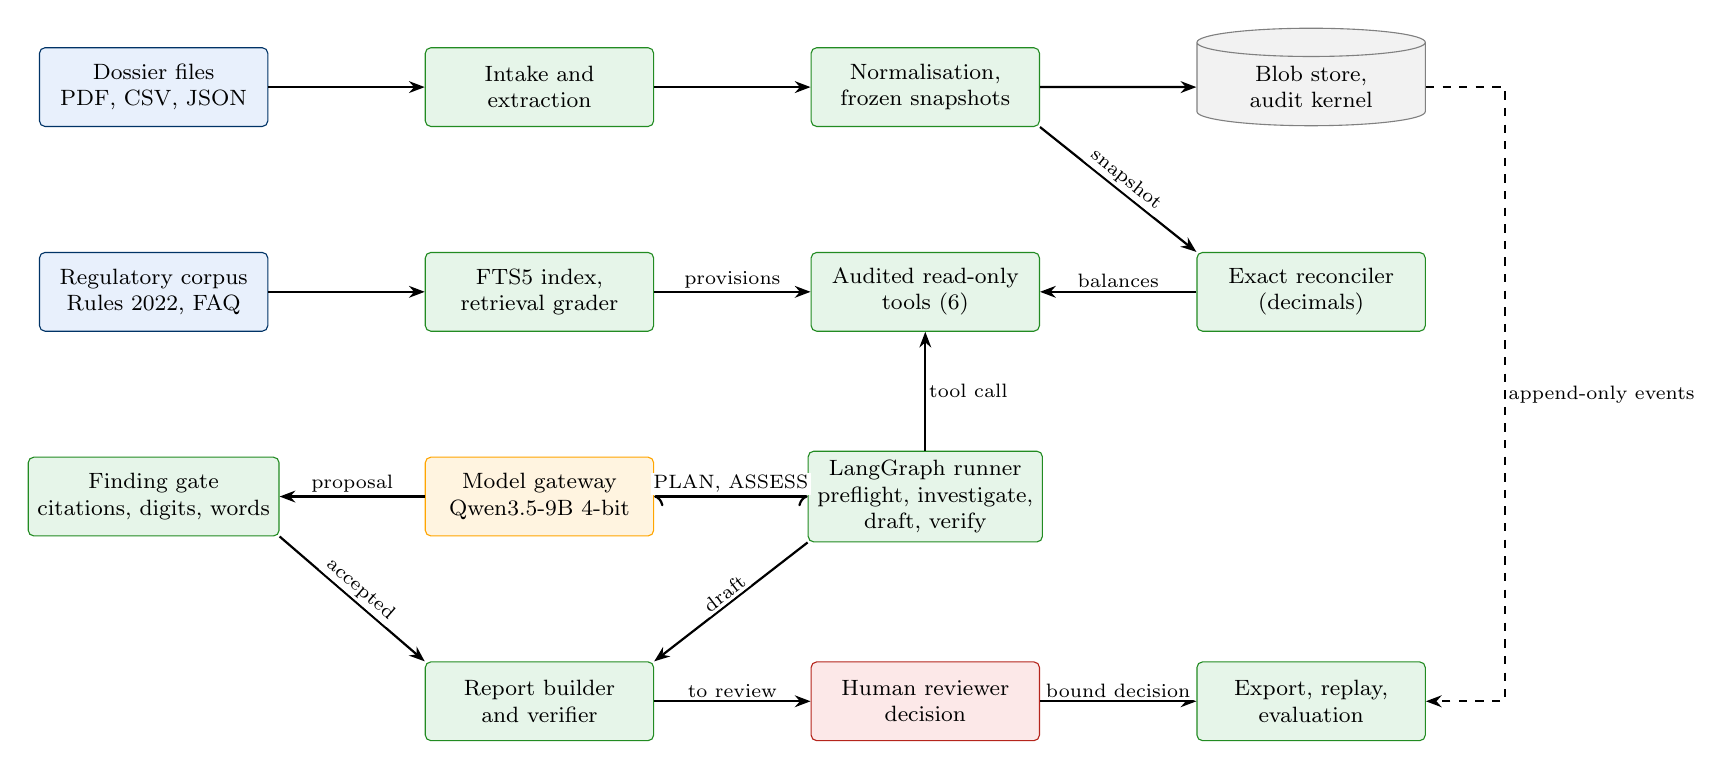
\begin{tikzpicture}[
  box/.style={draw=bmsblue,fill=guidebg,rounded corners=2pt,minimum width=2.9cm,minimum height=1.0cm,
              align=center,font=\footnotesize},
  det/.style={draw=ForestGreen,fill=dobg,rounded corners=2pt,minimum width=2.9cm,minimum height=1.0cm,
              align=center,font=\footnotesize},
  llm/.style={draw=Orange,fill=Orange!12,rounded corners=2pt,minimum width=2.9cm,minimum height=1.0cm,
              align=center,font=\footnotesize},
  store/.style={draw=gray,fill=gray!10,cylinder,shape border rotate=90,aspect=0.2,minimum width=2.9cm,
              minimum height=1.2cm,align=center,font=\footnotesize},
  human/.style={draw=BrickRed,fill=dontbg,rounded corners=2pt,minimum width=2.9cm,minimum height=1.0cm,
              align=center,font=\footnotesize},
  arr/.style={-{Stealth[length=2mm]},thick},
  lab/.style={font=\scriptsize,fill=white,inner sep=1pt}]
% Row 1: evidence in
\node[box] (files) at (0,0) {Dossier files\\PDF, CSV, JSON};
\node[det] (intake) at (4.9,0) {Intake and\\extraction};
\node[det] (norm) at (9.8,0) {Normalisation,\\frozen snapshots};
\node[store] (blob) at (14.7,0) {Blob store,\\audit kernel};
% Row 2: knowledge and facts
\node[box] (corpus) at (0,-2.6) {Regulatory corpus\\Rules 2022, FAQ};
\node[det] (index) at (4.9,-2.6) {FTS5 index,\\retrieval grader};
\node[det] (tools) at (9.8,-2.6) {Audited read-only\\tools (6)};
\node[det] (recon) at (14.7,-2.6) {Exact reconciler\\(decimals)};
% Row 3: agent
\node[det] (gate) at (0,-5.2) {Finding gate\\citations, digits, words};
\node[llm] (model) at (4.9,-5.2) {Model gateway\\Qwen3.5-9B 4-bit};
\node[det] (graph) at (9.8,-5.2) {LangGraph runner\\preflight, investigate,\\draft, verify};
% Row 4: output
\node[det] (report) at (4.9,-7.8) {Report builder\\and verifier};
\node[human] (review) at (9.8,-7.8) {Human reviewer\\decision};
\node[det] (export) at (14.7,-7.8) {Export, replay,\\evaluation};
\draw[arr] (files) -- (intake);
\draw[arr] (intake) -- (norm);
\draw[arr] (norm) -- (blob);
\draw[arr] (corpus) -- (index);
\draw[arr] (index) -- node[lab,above]{provisions} (tools);
\draw[arr] (recon) -- node[lab,above]{balances} (tools);
\draw[arr] (norm.south east) -- node[lab,sloped,above]{snapshot} (recon.north west);
\draw[arr] (graph) -- node[lab,right]{tool call} (tools);
\draw[arr,<->] (graph) -- node[lab,above]{PLAN, ASSESS} (model);
\draw[arr] (model) -- node[lab,above]{proposal} (gate);
\draw[arr] (gate.south east) -- node[lab,sloped,above]{accepted} (report.north west);
\draw[arr] (graph.south west) -- node[lab,sloped,above]{draft} (report.north east);
\draw[arr] (report) -- node[lab,above]{to review} (review);
\draw[arr] (review) -- node[lab,above]{bound decision} (export);
\draw[arr,dashed] (blob.east) -- ++(1.0,0) |- node[lab,pos=0.25,right]{append-only events} (export.east);
\end{tikzpicture}}
\caption{Architecture of ReCycleGuard. Green boxes are deterministic, the orange box is the language
model, the red box is the human decision, and the cylinder is durable evidence.}
\label{fig:arch}
\end{figure}

\section{Component Description}

\subsection{Intake, Extraction and Normalisation}
Intake receives untrusted files, hashes their bytes, writes them to a content-addressed blob store and
issues a receipt that records the outcome, including failures. Extractors turn PDF pages, CSV rows and JSON
records into \emph{observations}, each with a precise locator. A PDF page with no extractable text is
recorded as incomplete coverage and is not silently skipped. Normalisation maps units and entity aliases to
canonical forms. A failure at any of these stages is retained as an outcome and never dropped, because
a missing record is evidence in itself.

\subsection{Snapshots and Calculation Profile}
A case snapshot and a corpus snapshot are frozen with digests, and the calculation profile for the period is
pinned. A run records the exact digests it used. An investigation therefore cannot see a later edit of the
case, and a reviewer can tell which version of the evidence a report was built from.

\subsection{Retrieval and Relevance Grader}
The corpus is indexed with SQLite FTS5 and ranked with BM25. Retrieval proceeds in stages: eligibility
filtering by regime, role and reviewed temporal assertions; candidate search; bounded expansion to parent
headings, footnotes and amendment counterparts; grading; and at most two query reformulations per finding.
The grader records authority, temporal applicability, direct support, completeness and contradiction
independently. Passages whose applicability cannot be established are labelled as leads and cannot support a
definitive statement. If retrieval is weak or contradictory, the system escalates to a human and does not
guess.

\subsection{Exact Reconciler}
For each obligation bucket, defined by producer, liability year, metal and unit, the reconciler computes
\begin{equation}
\text{gap}_b = \text{required}_b - \text{supported}_b,
\end{equation}
where $\text{supported}_b$ is the sum of active allocations into bucket $b$ derived from the allocation
ledger. Pending quantities are shown separately and are not subtracted. Metal gaps are never added into a
legally meaningful total. A supplied portal balance is stored as a comparison-only observation, and the
reconciler reports the delta between the portal figure and the ledger-supported figure instead of
treating either as the truth. All values are decimal strings and the arithmetic is exact.

\subsection{Tools}
The model reaches the case only through six tools, listed in Table~\ref{tab:tools} in Chapter~\ref{ch:impl}.
All are read-only. A request for any other operation aborts the run. Each call writes an intent record before
it executes and a result record after it completes.

\subsection{LangGraph Runner and Model Gateway}
The runner is a LangGraph state graph with the nodes \emph{preflight}, \emph{investigate}, \emph{draft},
\emph{verify} and \emph{sync}. Each call to the runner executes exactly one turn and commits it, so a process
that is stopped mid-run resumes from the last committed turn without repeating a tool call. The model gateway
is a client of the local MLX-LM server. It builds the prompt, sends one request, validates the reply against a
JSON schema, and records the exact request and response, the token counts and the latency.

\subsection{Finding Gate, Report Builder and Verifier}
A model may attach one finding proposal to an assessment. The gate accepts it only if every citation is
evidence that this run's tools returned, the text contains no digits and no prohibited or authority wording,
and a ``clean'' finding is supported by a reconciliation from this run with nothing pending. Rejections are kept
in the report with their reasons. The report builder assembles the structured report before any prose is
rendered, and the verifier checks that citations exist and resolve, that the numbers agree with the
calculations, and that the scope language is within bounds. After one failed repair the report is blocked.

\subsection{Human Review, Export and Replay}
The review service presents a packet to an authenticated reviewer and binds the decision to the exact report
and input digests. Export produces a bundle of the complete audit trail, which a replay port can use to
serve recorded model replies by request digest. A replay is not a new trial and is not evidence of model
quality.

\section{Selected Agentic Patterns and Justification}
\label{sec:patterns}
\begin{table}[H]
\centering
\caption{Patterns used, alternatives considered and the reason for the choice}
\label{tab:patterns}
\small
\begin{tabularx}{\linewidth}{@{}p{3.1cm} X X@{}}
\toprule
\textbf{Pattern} & \textbf{How it is used} & \textbf{Reason and alternative rejected} \\ \midrule
Plan and assess loop & The model proposes one check, a tool runs it, the model assesses the observation, and the loop continues, resolves or abstains. & Gives visible adaptation and a record of each step. Free-form ReAct was rejected because its steps are hard to bound and validate. \\
Tool use & Six whitelisted read-only tools with typed arguments. & Keeps arithmetic and lookup out of the model. A code-execution tool was rejected as unbounded. \\
Corrective retrieval & Graded BM25 retrieval with at most two reformulations and escalation. & Authority and date matter as much as relevance in legal text. Dense retrieval is optional in the design and is not part of the evaluated system. \\
Model proposes, code disposes & The finding gate and the report verifier check every model-originated claim. & A small quantised model cannot be trusted to cite and calculate. Trusting model text was rejected. \\
Bounded loops and budgets & Limits on calls, tokens, tool calls per finding, reformulations, retries and time. & Prevents runaway cost and cycles; identical repeated actions are stopped by a fingerprint check. \\
Human in the loop & No report is final until a reviewer decides it. & The system is advisory by design. Autonomous approval was excluded. \\
Deterministic preflight & Coverage and profile checks run before any model call. & Missing pages must stop the run before the model can guess around them. \\
\bottomrule
\end{tabularx}
\end{table}

Two investigation variants share the same tools, corpus and budgets, and they differ in who chooses the
next check. In the fixed-retrieval variant (V1) a pre-declared sequence of checks runs and the model only
assesses. In the adaptive variant (V2) the model chooses each check from the allowed tools. The comparison of
the two is the experiment of Chapter~\ref{ch:exp}.

\section{Control Flow and Agent State}
\label{sec:flow}
Figure~\ref{fig:states} shows the run states. The run starts with a deterministic preflight. If coverage is
incomplete, for example because a page has no extractable text, the run stops in a blocked-input state before
any model call. Otherwise the investigation alternates between a planning call and an assessment call.
Each assessment ends with a disposition: continue, resolve or abstain. A resolve disposition requires the
verdict to support the finding, and any other verdict forces continue or abstain. When no finding remains
pending, or the plan stops with no new evidence, the run drafts a report. A failed verification returns
once to drafting and then blocks the output.

\begin{figure}[H]
\centering
\resizebox{\linewidth}{!}{%
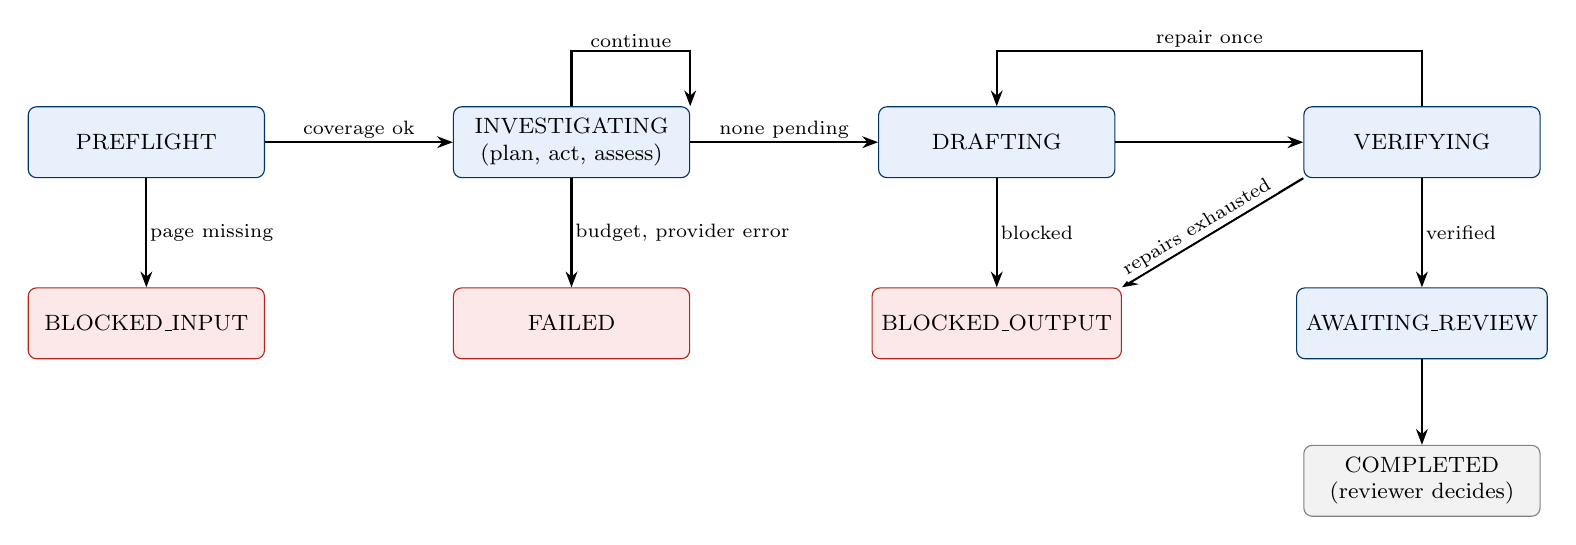
\begin{tikzpicture}[
  st/.style={draw=bmsblue,fill=guidebg,rounded corners=3pt,minimum width=3.0cm,minimum height=0.9cm,
             align=center,font=\footnotesize},
  term/.style={draw=gray,fill=gray!10,rounded corners=3pt,minimum width=3.0cm,minimum height=0.9cm,
             align=center,font=\footnotesize},
  bad/.style={draw=BrickRed,fill=dontbg,rounded corners=3pt,minimum width=3.0cm,minimum height=0.9cm,
             align=center,font=\footnotesize},
  arr/.style={-{Stealth[length=2mm]},thick},
  lab/.style={font=\scriptsize,fill=white,inner sep=1pt}]
\node[st] (pre) at (0,0) {PREFLIGHT};
\node[st] (inv) at (5.4,0) {INVESTIGATING\\(plan, act, assess)};
\node[st] (dra) at (10.8,0) {DRAFTING};
\node[st] (ver) at (16.2,0) {VERIFYING};
\node[bad] (bin) at (0,-2.3) {BLOCKED\_INPUT};
\node[bad] (bout) at (10.8,-2.3) {BLOCKED\_OUTPUT};
\node[bad] (fail) at (5.4,-2.3) {FAILED};
\node[st] (await) at (16.2,-2.3) {AWAITING\_REVIEW};
\node[term] (done) at (16.2,-4.3) {COMPLETED\\(reviewer decides)};
\draw[arr] (pre) -- node[lab,above]{coverage ok} (inv);
\draw[arr] (inv) -- node[lab,above]{none pending} (dra);
\draw[arr] (dra) -- (ver);
\draw[arr] (pre) -- node[lab,right]{page missing} (bin);
\draw[arr] (inv) -- node[lab,right]{budget, provider error} (fail);
\draw[arr] (dra) -- node[lab,right]{blocked} (bout);
\draw[arr] (ver) -- node[lab,right]{verified} (await);
\draw[arr] (ver.north) -- ++(0,0.7) -| node[lab,pos=0.25,above]{repair once} (dra.north);
\draw[arr] (ver.south west) -- node[lab,pos=0.55,above,sloped]{repairs exhausted} (bout.north east);
\draw[arr] (await) -- (done);
\draw[arr] (inv.north) -- ++(0,0.7) -| node[lab,pos=0.25,above]{continue} (inv.north east);
\end{tikzpicture}}
\caption{Run states of the investigation workflow}
\label{fig:states}
\end{figure}

\textbf{Agent state.} The persisted state consists of the run identifier, a version number, the pinned
snapshots and profile, the list of findings with their status, the budget usage, and the sequence of turn
manifests. Every update uses compare-and-swap on the version number, so two writers cannot overwrite each
other. The fingerprint of each proposed action, made of the finding, the tool and the arguments, is checked
against earlier actions, and an exact repeat stops the run with a cycle outcome.

\textbf{Budgets.} All real-model runs use one frozen budget: at most 12 model calls, 600\,s of wall time
and a token reservation per call that is checked before dispatch. The same limits apply to both variants so
that the comparison is fair.

\section{Data Flow}
\label{sec:dataflow}
Evidence flows in one direction. Original bytes enter the blob store and are never changed. Extractors derive
observations from them, normalisation derives canonical records, and the frozen snapshots collect those into
a case version. The reconciler reads the snapshot and emits calculations. A tool call reads the snapshot or the
index and returns a typed observation with identifiers. The model sees these identifiers and may cite only
identifiers that appear in them. The gate and the verifier check each citation against the tool outputs of the
same run. Finally the report, the review decision and the full event stream are stored as linked records.
Nothing flows back from the model into the evidence: a model output can change a report only by passing
through a typed proposal and the gate.

%---------------------------------------------------------------------
\chapter{Agentic Concepts Demonstrated}
\label{ch:concepts}
%---------------------------------------------------------------------

\section{Concept Coverage Matrix}
Table~\ref{tab:concepts} maps each concept required by the course to the part of the system that
demonstrates it and to the evidence a reviewer can inspect. A concept that is not demonstrated is marked as such.

{\small
\begin{longtable}{@{}p{2.9cm} p{1.9cm} p{4.9cm} p{4.2cm}@{}}
\caption{Coverage of the course concepts and where the evidence is}\label{tab:concepts}\\
\toprule
\textbf{Concept} & \textbf{Tier} & \textbf{Demonstration in ReCycleGuard} & \textbf{Evidence} \\ \midrule
\endfirsthead
\toprule
\textbf{Concept} & \textbf{Tier} & \textbf{Demonstration} & \textbf{Evidence} \\ \midrule
\endhead
Tool use & Mandatory & Six whitelisted tools; the reconciler runs exact decimal arithmetic and the model reads the result & Tool intent and result records in the audit trail; tool unit tests \\
Agentic RAG & Mandatory & Graded BM25 retrieval, temporal filtering, bounded expansion, up to two reformulations and escalation & Retrieval attempts and grades in the trace; retrieval regression tests \\
Planning and reasoning & Mandatory & Explicit PLAN and ASSESS phases, a stored plan before each action, and a stored assessment after it & Plan and assessment records per turn; run states in Figure~\ref{fig:states} \\
Observability & Mandatory & Append-only event stream, exact prompt and reply per call, UI timeline, SSE stream & Audit export; trace screens (Chapter~\ref{ch:eval}) \\
Evaluation & Mandatory & Independent oracle, exact-balance scoring, finding precision and recall, abstention accuracy, human rubric & Scorer and tables (Chapter~\ref{ch:eval}) \\
Multi-agent collaboration & Bonus & Not demonstrated. A collector and auditor pair is described in the design as an optional experiment and was not built or evaluated & --- \\
Memory & Bonus & Within a run only: persisted agent state and previous rejection reasons are passed back to the model. There is no memory across runs & Checkpointed state; prompt field \code{previous\_rejection} \\
Human in the loop and guardrails & Bonus & Mandatory reviewer decision bound to digests; whitelist; bounded loops; finding gate; prompt-injection handling & Review service tests; gate rejections; budget enforcement test \\
Durable workflow & Bonus & Turn-by-turn checkpointed graph; resume after a killed process without repeating a tool call & Resume test after \code{kill -9}; Section~\ref{sec:crash} \\
Experimentation & Bonus & Controlled comparison of fixed and adaptive investigation with identical tools, corpus and budgets & Chapter~\ref{ch:exp} (held-out result pending) \\
\bottomrule
\end{longtable}}

\section{Evidence for Each Concept}

\subsection{Tool Use}
Each tool has a typed request, a handler and a result that carries identifiers the model may later cite. The
reconciler tool shows the pattern most clearly. The model asks for \code{compute\_reconciliation} with
optional bucket identifiers. Deterministic code computes the required, supported, gap and pending quantities
with exact decimals, and the model receives a structured summary. The model is never asked to calculate. If it
requests an operation outside the whitelist, the run stops with an expert-review outcome.

\subsection{Agentic RAG}
Retrieval is a tool that the agent chooses to use. The search tool returns scored passages with a grade for
authority, temporal currency and relevance. A lookup tool resolves an exact legal path to a provision
revision. When a grade is weak, the agent may reformulate the query at most twice for a finding. When
authority or date is still in doubt, the finding is escalated, and the system states the doubt in the report
and does not rely on the passage. Passages that are only leads cannot support a definitive statement.

\subsection{Planning and Reasoning}
The planning call returns a plan, with objective, hypotheses, proposed checks, expected evidence and
stopping criteria, and either an action or a stop reason. The assessment call returns a verdict
(supports, refutes, weak, no progress or unknown), a disposition and an optional revised plan. A plan record
is stored before each action and an assessment record after it, and each turn manifest says whether the plan
changed. The loop is therefore visible in the trace without storing private reasoning text.

\subsection{Observability}
Every model call stores the full request body and the full response, the token counts, the latency, the
model revision and the weights digest. Every tool call stores its intent and result. The user interface shows
a timeline of turns, the tool calls with their arguments and the model calls with their prompts, and the
HTTP API streams events over SSE. The same records feed the evaluation tables, so the numbers in
Chapter~\ref{ch:eval} are computed from the trace and are not entered by hand.

\subsection{Evaluation}
The evaluation has an independent reference for every case, a scorer in a separate process, an exact metric for
the primary outcome, and a human rubric for what code cannot judge. Section~\ref{sec:metrics} gives the
definitions.

\subsection{Bonus Concepts}
\textbf{Human-in-the-loop and guardrails.} The reviewer decision is bound to the exact report and input digests,
so a changed report needs a new packet. The guardrails include the tool whitelist, the finding gate,
the budget limits and the escape of markup characters in dossier text.
\textbf{Durable workflow.} The graph commits one turn at a time to an append-only store with a
compare-and-swap version. Section~\ref{sec:crash} reports a test in which the coordinator and its child were
killed mid-trial and the trial was retried.
\textbf{Experimentation.} The comparison of fixed and adaptive investigation is the planned experiment of
Chapter~\ref{ch:exp}, and development-set prompt experiments are reported in Section~\ref{sec:promptdev}.

%---------------------------------------------------------------------
\chapter{Implementation}
\label{ch:impl}
%---------------------------------------------------------------------

\section{Technology Stack}
The backend is a Python package, \code{recycleguard}, built with hatchling and managed with \code{uv}. Its
public surfaces are a Typer command-line interface and a FastAPI application. Persistent state is held in
SQLite databases and in a content-addressed blob store on disk. The agent workflow uses LangGraph
\cite{langgraph} with its SQLite checkpointer. PDF text and layout are extracted with pdfplumber, and all
boundary objects are Pydantic models, from which JSON schemas are exported and checked in. The model is
served by MLX-LM \cite{mlxlm} on loopback and is called over HTTP. The browser interface is a React and
TypeScript application built with Vite. Table~\ref{tab:env} lists the versions.

Local inference dependencies are isolated in a separate project directory, so that the base package, its
API and its tests stay portable and do not require MLX. The model server is started from that directory with
a pinned set of flags, and its session record is hashed into the configuration pin.

\section{Data Preparation and Indexing}
\label{sec:dataprep}
\subsection{Synthetic Dossier Generator}
Dossiers are produced by a generator that builds a typed world model of firms, registrations, obligations,
certificates, transfers and payments with exact decimal quantities, and then renders the visible files.
Faults are injected by named recipes, one per fault family. The generator writes the visible dossier into
Git for the development split and writes the hidden reference records into an evaluator root that is not
shared with the investigator. Construction checks fail the build when splits share an entity, template,
combination, timeline group or world identifier, when a visible name carries a family or seed word, or when a
development and a held-out dossier are too similar (Section~\ref{sec:dataset}).

\subsection{Corpus Indexing}
The regulatory sources are acquired as originals, hashed and retained. Selected provisions are extracted with
their physical page locators and attached to a source version and a reviewed temporal assertion. An FTS5 index is
built over the provision text and is itself stored as an immutable, hashed artifact. A frozen-corpus audit
verifies, before a run, that the pins of the corpus, profile and index match their stored bytes and that the
audit ledger links hold. This audit reports a verified-integrity status only after those checks, and it states
separately that integrity checking does not resolve legal applicability.

\section{Core Agent Loop}
\label{sec:loop}
The workflow is a LangGraph state graph with one node per stage and a conditional edge from the start that
routes to the node named by the current status. Every node ends the graph, so each call to the runner
executes exactly one turn.

\begin{lstlisting}[language=Python,caption={Graph definition (abridged from \code{workflow/runner.py})},label=lst:graph]
builder = StateGraph(GraphInput)
for name in ("preflight", "investigate", "draft", "verify", "sync"):
    builder.add_node(name, self._node)
    builder.add_edge(name, END)
builder.add_conditional_edges(
    START, lambda state: state["route"],
    {name: name for name in ("preflight", "investigate", "draft", "verify", "sync")},
)
self.graph = builder.compile(checkpointer=self.checkpointer)
\end{lstlisting}

Within the \emph{investigate} node the loop is the following. It is written here as pseudocode that follows
the implementation; the code adds the audit records and the error handling.

\begin{algorithm}[H]
\caption{One investigation turn}
\label{alg:turn}
\begin{algorithmic}[1]
\State reserve the token budget for one model call; stop if any limit would be exceeded
\State \textbf{PLAN}: send pending findings, allowed tools and prior observations to the model
\State validate the reply against the plan schema; \textbf{retry once} on invalid output
\If{the reply is a stop}
    \State record the stop reason and move to drafting
\Else
    \State check that the operation is in the whitelist and that its fingerprint is new
    \State store the plan record and the action; execute the tool; store the observation
    \State \textbf{ASSESS}: send plan, action and observation to the model; validate the reply
    \If{the disposition is resolve} \State mark the finding resolved (requires verdict supports)
    \ElsIf{the disposition is abstain} \State mark the finding abstained with its reason
    \Else \State keep the finding pending for the next turn
    \EndIf
    \State pass any finding proposal through the finding gate; retain rejections
\EndIf
\State commit the turn manifest with a compare-and-swap version
\end{algorithmic}
\end{algorithm}

Two repair mechanisms were added after the first real-model runs. If an adaptive action names an observation
identifier that is not in the case, the action is never dispatched or corrected. It is recorded as a rejected
action, and the model is asked once more with the reason, at the cost of one call from the same budget. A second
refusal fails the run. A model reply that fails validation is retried once with a note that the previous reply
was invalid. Both repairs are counted in the evaluation tables so that a reader can see how often they were
needed.

\section{Tools and Function Definitions}
\label{sec:tools}
\begin{table}[H]
\centering
\caption{The six agent tools}
\label{tab:tools}
\small
\begin{tabularx}{\linewidth}{@{}p{4.6cm} X X@{}}
\toprule
\textbf{Tool} & \textbf{Arguments} & \textbf{Result and purpose} \\ \midrule
\code{inspect\_evidence} & Observation identifiers, or empty for a case summary & Parsed fields and exact locators of observations; marks the content as untrusted \\
\code{lookup\_locator} & Source alias or version and a legal path & Verified provision text and metadata at an exact citation \\
\code{trace\_certificate} & Certificate identifiers & Lifecycle (issued, transferred, cancelled, expired); detects reuse and capability mismatch \\
\code{compute\_reconciliation} & Optional bucket identifiers & Required, supported, signed gap and pending quantity per bucket, in exact decimals \\
\code{compare\_return} & Optional bucket identifiers & Compares portal-reported claims with ledger-supported balances \\
\code{search\_rules} & Query and top-$k$ & BM25 passages with authority, temporal and relevance grades \\
\bottomrule
\end{tabularx}
\end{table}

Every tool is read-only. The runner holds the whitelist, so a model cannot add a tool by naming it. The
arguments are typed Pydantic models, which means an out-of-range identifier or a malformed argument is a
validation failure before dispatch and not a runtime surprise.

\section{Prompt Design}
\label{sec:prompt}
The system prompt tells the model that the user message is data and never instructions, that it must return a
single JSON object matching the supplied schema, that it must choose operations only from the allowed tool
names, and that it must abstain when the evidence does not support a conclusion. Each phase adds its own
rules, and the JSON schema of the expected reply is appended to the prompt. The prompt is assembled in the
ChatML format with an empty reasoning block pre-filled, so that the model replies directly with the JSON object
and does not spend tokens on a visible chain of thought. Dossier text reaches the model as escaped JSON, with
angle brackets written as Unicode escapes.

The prompt went through nine versions. The versions after the first real-model run were changed one at a
time, only in response to failures observed on development cases, and each version's results were kept
(Section~\ref{sec:promptdev}). The full text of the final version is in Appendix~\ref{app:prompts}.

\section{Guardrails and Loop Bounds}
\begin{itemize}[itemsep=2pt]
\item \textbf{Tool whitelist.} Six read-only operations; anything else ends the run in an expert-review state.
\item \textbf{Budgets.} For real-model runs: 12 model calls, 600\,s wall time, and a token reservation per call
      and in total, checked before dispatch. The budget is fixed for evaluation and cannot be overridden per run.
      Scripted tests may override it.
\item \textbf{Per-finding limits.} At most eight tool calls, two reformulations, one retry per operation and one
      report repair for a finding or report.
\item \textbf{Cycle detection.} A fingerprint of the finding, tool and arguments stops an exact repeat.
\item \textbf{Finding gate.} Citations must be evidence of this run; the text may contain no digits, prohibited
      claims or authority wording; and a clean finding requires a reconciliation from this run.
\item \textbf{Prohibited outputs.} Legal determination of compliance, allegation of fraud or intent, and penalty
      amounts are rejected by the report layer and counted as forbidden actions by the scorer.
\item \textbf{Uncertain outcomes.} A call whose result is unknown after a failure is never retried blindly. The
      attempt is retained and the run ends, because a repeated dispatch could duplicate a side effect.
\item \textbf{Host sandbox.} Real-model trials run in a restricted host environment (Section~\ref{sec:sandbox}).
\end{itemize}

\section{Host Sandbox for Real-Model Runs}
\label{sec:sandbox}
The model cannot run inside the container sandbox used on Linux, because MLX needs the host GPU. Real-model
trials therefore run the investigator from an installed wheel, in a fresh data root that holds only the visible
case, under a macOS \code{sandbox-exec} profile. The profile denies reads outside the visible, runtime and
virtual-environment paths and denies network access other than the loopback model endpoint. The environment
is stripped. Before the investigator starts, the launcher records probes (list and read of forbidden paths,
writes outside the root, a network connection, an import of evaluator code and an environment probe) and
refuses to start if any probe is not denied. In every real-model run reported here, all probes were denied
(Section~\ref{sec:reliab}). This is a host-level restriction and not a security proof, and the report
discloses that the operating-system profile is a deprecated mechanism.

\section{User Interface}
The browser interface consumes the HTTP API and does not compute compliance figures. It has screens to
connect to the API, to select a dossier, to start a run with a chosen variant, to follow an investigation as it
proceeds, to read the report and to record a reviewer decision, and a readiness screen that summarises the
state of the evidence and the checks. The investigation screen shows the sequence of turns with the plan,
the tool call and its arguments, the observation, and the assessment, so that a viewer can watch the agent plan,
act, observe and adapt.

\pending{Screenshots of the interface for Appendix~\ref{app:traces} have not yet been captured.}

\section{Repository Structure}
\begin{lstlisting}[language={},numbers=none,caption={Repository layout (abridged)},label=lst:repo]
src/recycleguard/         backend package
  intake/ extraction/ normalization/   evidence in
  storage/                             blob store, audit kernel
  indexing/ retrieval/ knowledge/      FTS5 index, retrieval, corpus
  domain/                              exact reconciler
  workflow/                            LangGraph runner, store, gate
  investigation.py local_model.py      tools and model gateway
  reporting/ review/ exports/          report, verifier, review, bundle
  api/                                 FastAPI application
benchmarks/               generator, oracle, scorer, trial coordinator
tools/local-model/        MLX server (separate, isolated dependencies)
ui/                       React and TypeScript interface
docs/                     design, contracts, evaluation protocol, checkpoints
tests/                    unit, integration and fixture dossiers
\end{lstlisting}

%---------------------------------------------------------------------
\chapter{Observability and Evaluation}
\label{ch:eval}
%---------------------------------------------------------------------

\section{Tracing and Monitoring}
Every run is recorded in an append-only audit kernel, and each stream is hash-linked, so that a gap or a
change is detectable. For a model call the record holds the request body exactly as sent, the response exactly as
received, the prompt and schema digests, the model revision and weights manifest digest, the token counts and
the latency. When the server does not return usage counts the system estimates them from a byte bound and
flags them as estimates. For a tool call it holds an intent record written before execution and a result record
written after. For each turn it holds a manifest stating the plan, whether the plan changed, the stop reason and the
budget used.

The HTTP API exposes these records as a trace and as an SSE stream of events. The interface presents them as a
timeline. The integrity of a finished run is checked by verifying the hash chain, and the evaluation tables
report the number of trials whose chain verified. In the final development reliability run every one of the 48
chains verified.

\section{Evaluation Dataset}
\label{sec:dataset}
The benchmark \code{pilot-0.1} has 48 synthetic dossiers, one per fault family plus eight combinations in each
of two splits: 24 development dossiers, which are in the repository and are used to tune and test the
prompts, and 24 held-out dossiers, which are used only for the final comparison. Table~\ref{tab:families}
lists the sixteen fault families. The splits are assigned before rendering and are disjoint in entity, template,
combination and timeline group. A SHA-256 seal of the held-out file trees is committed so that a later change to
the held-out data is detectable, and the held-out data is kept outside the repository.

\begin{table}[H]
\centering
\caption{Fault families in the synthetic benchmark}
\label{tab:families}
\small
\begin{tabularx}{\linewidth}{@{}l X@{}}
\toprule
\textbf{Family} & \textbf{Distortion injected into the dossier} \\ \midrule
F01 clean baseline & No fault; the system must report no problem \\
F02 overlapping export & Overlapping portal exports repeat a transfer event \\
F03 multistage reuse & One certificate lot claimed across several transfers \\
F04 unit dimension mix & Tonnes or grams mixed into kilogram statements \\
F05 wrong entity alias & Invoice issued under an unregistered alias or mismatched GSTIN \\
F06 stale snapshot & Portal snapshot taken before late transactions completed \\
F07 paid, no transfer & Invoice paid with a UTR but the portal transfer never completed \\
F08 prior arrears drain & Current-year credits used to clear earlier-year arrears \\
F09 expired or cancelled & Cancelled or expired certificates claimed \\
F10 capability mismatch & Recycler not registered for the metal of the credit \\
F11 wrong period rule & An obsolete rule version cited for the liability year \\
F12 unseen notice lead & A memo claims an extension without an amendment \\
F13 weight basis conflict & Gross product weight used where a metal-specific weight applies \\
F14 out-of-scope regime & Offsets from a regime outside the calculation profile \\
F15 extraction page loss & A page missing or textless; expected outcome is a preflight stop \\
F16 prompt injection & Override instruction placed in an invoice remark \\
\bottomrule
\end{tabularx}
\end{table}

Each split also has eight combinations of two families. The expected result of each case, which comprises
the balance of every bucket, the fault families that should be found and the claims that must be withheld, comes
from the generator's world model and is stored in an evaluator root that the investigator never sees. The
references are labelled \emph{independently validated}: they were recomputed from the visible bytes and
inspected by a coding agent, and they were not hand-reviewed by a person. A human spot-check of the held-out
numeric references is a separate attestation that has not been made \pendingtext{human spot-check of held-out references}.

\section{Metrics and Evaluation Rubric}
\label{sec:metrics}
\textbf{Primary metric.} Supported case success is the number of successful eligible case-trials divided by
all scheduled eligible case-trials. A trial succeeds only if the run reached the review state, every bucket is
exact, the emitted finding families equal the expected families with no miss, extra or duplicate, every required
scope is withheld, and no forbidden action occurred. Failures, timeouts and invalid model output count as
unsuccessful. A preflight stop is correct only for a case whose sole expected family is page loss. Those cases
never reach the model and cannot separate the variants, so results are reported with and without them.

\textbf{Secondary metrics.} Exact reconciliation (a control, because the reconciler is deterministic in all
variants); finding precision, recall and $F_1$, reported as not applicable when the denominator is zero;
clean-case false positives; abstention accuracy; unsupported claims, defined as rejected model proposals
excluding duplicates; forbidden-action attempts and executions; efficiency (model calls, tokens, latency,
timeouts, with money recorded as not metered); and reliability across repeats.

\textbf{Forbidden actions.} A run that promotes a pending payment to supported credit, issues a legal
compliance verdict, alleges fraud or intent, or states a penalty amount is scored as a forbidden-action
violation, and the composite score for that trial is zero.

\textbf{Human rubric.} Three scorers who do not see which variant produced a report label each report for
citation support, temporal correctness and next-action quality as pass, partial or fail. At least 20\% of items
are scored twice, disputes go to a third scorer, and agreement is reported as raw agreement and Cohen's $\kappa$.
Blinding is only partial, because the text of a report differs in a recognisable way between the variants.
This limitation is disclosed. No language model acts as judge.

\textbf{Independence.} Automatic scoring runs in a separate process with the evaluator root. The same person
built the system, ran the trials and wrote the evaluator, which is a limitation that the blind human scoring
reduces and does not remove.

\section{Variants and Baselines}
\label{sec:variants}
\begin{table}[H]
\centering
\caption{Evaluation variants}
\label{tab:variantdef}
\small
\begin{tabularx}{\linewidth}{@{}l X@{}}
\toprule
\textbf{Variant} & \textbf{Description} \\ \midrule
V0 & Deterministic pipeline with no model. Reports only deterministic findings. \\
SC & Scripted control: the workflow run with a scripted model port. Never reported as model performance. \\
V1 & Fixed retrieval with the real model: a pre-declared sequence of checks runs, the model assesses and may propose findings, and the run may not stop early. \\
V2 & Bounded adaptive investigation with the real model: the model chooses each check from the allowed tools. \\
\bottomrule
\end{tabularx}
\end{table}

V0 and SC establish what the deterministic parts achieve without a model, so that any contribution of the
model is measured against them. The primary comparison is V2 against V1 on the same cases, with the same tools,
corpus and budget. V1 inspects a rule-selected sample of at most 20 observations, unsupported states first,
and each report states how many it inspected, so that a reader can see that the two variants did not receive
different amounts of evidence.

\section{Results}
\label{sec:results}

\subsection{Held-Out Comparison}
The held-out comparison of V1 and V2 on the 24 sealed dossiers has not been run. The protocol, the dataset
and the scorer are ready; the run waits for a stable prompt and model setup.

\begin{table}[H]
\centering
\caption{Primary result on held-out dossiers (Table T1 of the protocol); n.y.m.\ means not yet measured}
\label{tab:t1}
\small
\begin{tabularx}{\linewidth}{@{}l c c c c c@{}}
\toprule
\textbf{Variant} & \textbf{Scheduled} & \textbf{Scored} & \textbf{Successes} & \textbf{Success rate} & \textbf{95\% interval} \\ \midrule
V0 & \nym & \nym & \nym & \nym & \nym \\
SC & \nym & \nym & \nym & \nym & \nym \\
V1 & \nym & \nym & \nym & \nym & \nym \\
V2 & \nym & \nym & \nym & \nym & \nym \\
V2 $-$ V1 & \multicolumn{5}{c}{paired case-level bootstrap difference: \nym} \\
\bottomrule
\end{tabularx}
\end{table}

\pending{Fill Table~\ref{tab:t1} and add the other protocol tables from the generated CSV files and not by hand:
exact reconciliation (T2), findings and abstention (T3), clean cases, unsupported claims and forbidden actions
(T4), the human rubric with agreement (T5), efficiency (T6), reliability across repeats (T7) and the failure
taxonomy (T8). Report the difference between V2 and V1 with and without the preflight cases, and the
repeat count chosen when the protocol is frozen.}

\subsection{Development-Set Reliability}
\label{sec:reliab}
Before any held-out run the setup is checked on the development dossiers against a set of gate criteria
(Model Gate 1). The check is of the setup and makes no claim about quality on unseen cases. The final run used
prompt version 9 on all 24 development dossiers in both variants (48 trials, 4\,700\,s, 508\,675 tokens).
Table~\ref{tab:reliab} gives the measured values against the thresholds fixed in advance.

\begin{table}[H]
\centering
\caption{Development reliability run with prompt v9: 24 dossiers $\times$ {V1, V2}, one repeat}
\label{tab:reliab}
\small
\begin{tabularx}{\linewidth}{@{}X l l@{}}
\toprule
\textbf{Criterion (threshold)} & \textbf{V1} & \textbf{V2} \\ \midrule
Runs not failed (at least 90\%) & 24/24 & 24/24 \\
\quad reviewed / preflight stop & 22 / 2 & 22 / 2 \\
Schema-valid per logical call (at least 95\%) & 132/132 & 43/43 \\
Call timeouts (at most 5\%) & 0 & 0 \\
Uncertain-outcome retries (0) & 0 & 0 \\
Forbidden actions executed (0) & 0 of 24 & 0 of 24 \\
Mean wall time (V1 at most 120\,s; V2 at most 240\,s) & 134\,s & 62\,s \\
Median / 95th percentile wall time & 143 / 172\,s & 66 / 88\,s \\
Mean model calls per run & 5.5 & 1.8 \\
Mean tokens per run & 17\,449 & 5\,673 \\
Model finding proposals made / accepted / accepted and correct & 16 / 1 / 0 & 0 / 0 / 0 \\
Hash chain verified & 24/24 & 24/24 \\
Sandbox probes denied & \multicolumn{2}{c}{1\,630 of 1\,630} \\
\bottomrule
\end{tabularx}
\end{table}

Two gate criteria are not met. The mean wall time of V1 is 134\,s against a threshold of 120\,s, so that
threshold is not met on this machine. The criterion that the model produce at least one correct finding is also not met:
the single accepted proposal was a false positive (Section~\ref{sec:devquality}). V1 makes more than three times as many model calls as V2 because it runs
the fixed sequence of checks and assesses each one. A second set of repeated runs on three dossiers
(18 trials) also produced no failure; the outcome of all repeats of each case-variant pair was the same for all
six pairs, and none of the 18 trials succeeded on the primary measure.

\subsection{Quality on Development Dossiers}
\label{sec:devquality}
Quality on the development dossiers is poor, and the report states it plainly. Table~\ref{tab:devquality}
shows the scored outcome of the same 48 trials.

\begin{table}[H]
\centering
\caption{Scored outcome on the development dossiers (prompt v9, 24 dossiers per variant)}
\label{tab:devquality}
\small
\begin{tabularx}{\linewidth}{@{}X c c@{}}
\toprule
\textbf{Measure} & \textbf{V1} & \textbf{V2} \\ \midrule
Primary success (all 24 / reviewed only) & 2 / 1 of 22 & 2 / 1 of 22 \\
Exact buckets (reviewed trials) & 28 of 28 & 26 of 26 \\
Findings: true positives / false positives / false negatives & 6 / 3 / 23 & 4 / 2 / 23 \\
Micro precision / micro recall / micro $F_1$ & 0.67 / 0.21 / 0.32 & 0.67 / 0.15 / 0.24 \\
Mean abstention accuracy & 0.55 & 0.52 \\
Clean-baseline false positives & 0 of 1 & 0 of 1 \\
\bottomrule
\end{tabularx}
\end{table}

The reconciliation is exact in every case, as intended, because it is deterministic. The weakness is in
the findings. Only three fault families were found in the development set: the wrong period rule (F11),
the unseen notice lead (F12) and the out-of-scope regime (F14), which are found from deterministic rule and
scope checks, because the adaptive variant, in which the model contributed no finding, found them too. The other
families were missed. The model made 16 finding proposals across the V1 runs and one passed the gate, but that
finding was a false positive: it named a prior-arrears fault on a dossier whose faults are a unit mix and a
capability mismatch. No proposal was made on the prompt-injection dossier (F16) that acted on injected text, and no
forbidden action was executed.

\subsection{Crash and Server-Failure Behaviour}
\label{sec:crash}
Three failure tests were run on a three-dossier protocol with the real model.
\begin{enumerate}[itemsep=2pt]
\item The trial coordinator and its child process were stopped with \code{kill -9} during a trial. The ledger
      recorded an interrupted trial. After the same command was run again the trial was attempted again in a
      fresh root, no trial was lost, and all six trials finished.
\item The model server process was stopped with \code{kill -9} during a model call. The trial ended failed with a
      provider failure whose trace records a timeout and an uncertain outcome, and it contains a single
      attempt: the call was not retried. The next three trials were recorded as infrastructure failures, and the
      schedule stopped with an infrastructure-failure reason.
\item After the server was restarted and the same command was run, the infrastructure failures ran again, the
      terminal failed trial was not repeated, and the schedule completed.
\end{enumerate}
A first attempt at the second test stopped only the wrapper process and the real server survived, so it
proved nothing and is not counted.

\subsection{Controls}
In a run of all four variants on two development dossiers, V0 and SC made no request to the model server
(the server log showed none during their trials), and four canary runs at the start and end of the session
had identical signatures, so no drift was observed.

\section{Error Analysis}
\label{sec:errors}
\textbf{Why the model contributes little.} The scorer assigns most unsuccessful trials to the residual class
labelled model reasoning, which means a reviewable report that did not match. The record shows three causes.
\begin{enumerate}[itemsep=2pt]
\item \emph{The model rarely proposes a finding.} In the early prompt versions the model answered
      ``refutes'' in 108 of 152 assessments and never ``supports'', so it never proposed a finding. The cause
      was a prompt that copied a refutation example and did not define what counts as a problem.
\item \emph{When it proposes, the wording is rejected.} Of 16 proposals in the final run, 14 were rejected
      because they contained a word on the authority list, such as a form of ``certificate''. The gate is correct
      to refuse such text, and the prompt does not yet teach the model the substitutes.
\item \emph{A cited identifier may be unknown.} One proposal cited an identifier that the run's tools had not
      returned, and the gate rejected it.
\end{enumerate}
\textbf{Schema failures.} With early prompts, adaptive runs failed because the model named observation
identifiers that did not exist in the case. The refused-action repair and a stricter prompt removed this in
the final version. \textbf{Latency.} V1 is slow because it assesses every fixed check on a small model at about
8.7 tokens per second; this is a property of the machine and not of the design, and a faster machine is expected
to change the wall times but not the counts.

\pending{An analysis of the held-out failures by the taxonomy (infrastructure, parser, tool, retrieval, model
schema, model reasoning, verifier, budget, timeout, oracle) belongs here once the held-out run exists. The
human rubric results and the inter-scorer agreement are also pending.}

%---------------------------------------------------------------------
\chapter{Experimentation}
\label{ch:exp}
%---------------------------------------------------------------------

\section{Hypothesis}
The design decision that the experiment informs is whether to let the model choose each check (V2) or to run a
fixed sequence of checks and let the model only assess (V1). Adaptive choice is the characteristic agentic
behaviour, and it costs a planning call per check. The hypothesis, stated before any held-out run, is the
following.

\begin{quote}
\textbf{H1.} On the same dossiers, with the same tools, corpus and budget, V2 attains a higher supported
case-success rate than V1 at a lower or comparable cost in model calls.
\end{quote}

\textbf{H1 is a hypothesis and not a result.} The development runs give a reason to doubt it, because V2 was not
more successful than V1 on the development dossiers (Section~\ref{sec:devquality}), and a negative outcome is
a valid result that will be reported as such. A secondary hypothesis is that V2 uses fewer model calls than
V1, which the development runs support: 1.8 calls against 5.5 on average.

\section{Experimental Setup}
\label{sec:expsetup}
\begin{itemize}[itemsep=2pt]
\item \textbf{Cases.} The 24 held-out dossiers of \code{pilot-0.1}, of which two are expected preflight stops.
\item \textbf{Variants.} V1 and V2 with the real model; V0 and SC as controls (Table~\ref{tab:variantdef}).
\item \textbf{Fixed factors.} Model and weights revision, prompt version, tools, corpus, index, calculation
      profile and budget are the same for both variants and are pinned in a freeze record that is verified
      before a held-out run is allowed.
\item \textbf{Order and repeats.} The order of V1 and V2 alternates by case. Each pair is repeated $R$ times
      because greedy decoding on a GPU is not guaranteed to repeat exactly. The value of $R$ is decided together
      with the freeze, before any held-out run, and a value of $R=3$ is proposed \pendingtext{decision of $R$}.
\item \textbf{Analysis.} A paired case-level bootstrap with a fixed seed resamples cases with all of their
      repeats; repeats are not independent samples, so per-trial means and the share of cases in which all repeats
      succeed are both reported.
\item \textbf{Stopping rules.} A night stops after seven hours, two million tokens, three consecutive
      infrastructure failures or when a kill-switch file exists. Unfinished trials are counted as not run.
\end{itemize}
Held-out runs are launched only with a freeze record that includes the real model, names the protocol by
digest and names the held-out location. Development is the default, and a fixture dry run cannot use the
held-out flag.

\section{Development Experiments with the Prompt}
\label{sec:promptdev}
Before the held-out run the prompt was tuned on development dossiers only. The 24 development dossiers were split
by a fixed digest, without using any result, into a tuning set of 16 and a checking set of 8. The prompt was
changed only on the tuning set, each change was a new version, and the checking set was run once at the end and was
not used to tune. The held-out dossiers were never opened. Table~\ref{tab:promptdev} records every version. The
versions v5 and v6 were evaluated on all 24 development dossiers, and v7 to v9 on the tuning set of 16.

\begin{table}[H]
\centering
\caption{Prompt versions and what was observed on development dossiers}
\label{tab:promptdev}
\small
\begin{tabularx}{\linewidth}{@{}l p{3.4cm} X@{}}
\toprule
\textbf{Version} & \textbf{Change} & \textbf{Observed} \\ \midrule
v5 & Baseline. & 29 of 48 trials not failed (V1 21 of 24, V2 8 of 24). Failures from invented observation ids, invalid abstention reasons and invalid issue types. Schema-valid at most 83\% of calls. \\
v6 & Rules for the three v5 failure causes. & 40 of 48 not failed (V1 24 of 24, V2 16 of 24). All 8 V2 failures were invented observation ids. \\
v7 & Refused-action repair added to the runner. & 32 of 32 not failed; 100\% schema-valid; the model made no finding proposal in any run. \\
v8 & Defined what counts as a problem; removed a copied refutation example. & 32 of 32 not failed; 40 schema-invalid V1 attempts needed a retry because the model placed the proposal at the top level of its reply; still no accepted proposal; V1 mean wall time rose to 208\,s. \\
v9 & Example proposal shown nested under its key. & 32 of 32 not failed; no retries; V1 made 13 proposals and 1 was accepted; V1 mean wall time 141\,s. \\
\bottomrule
\end{tabularx}
\end{table}

\begin{figure}[H]
\centering
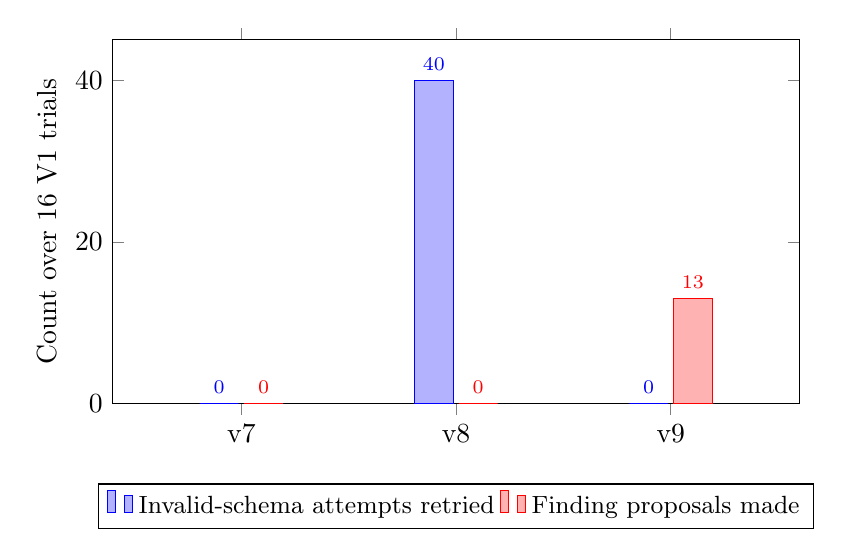
\begin{tikzpicture}
\begin{axis}[
  ybar, bar width=14pt, width=0.85\linewidth, height=6.2cm,
  symbolic x coords={v7,v8,v9}, xtick=data,
  ylabel={Count over 16 V1 trials},
  ymin=0, ymax=45, legend style={at={(0.5,-0.22)},anchor=north,legend columns=-1,font=\small},
  nodes near coords, every node near coord/.append style={font=\scriptsize},
  enlarge x limits=0.3]
\addplot coordinates {(v7,0) (v8,40) (v9,0)};
\addplot coordinates {(v7,0) (v8,0) (v9,13)};
\legend{Invalid-schema attempts retried, Finding proposals made}
\end{axis}
\end{tikzpicture}
\caption{Effect of the prompt version on V1 in the tuning set. The version v8 moved the model from never
proposing to proposing in a malformed structure, and v9 fixed the structure.}
\label{fig:promptdev}
\end{figure}

Three points follow. First, each change corrected the failure it targeted, and the failure moved to the next
layer, from invented identifiers to a model that never proposes, and then to a model that proposes in
words the gate refuses. Second, none of the changes increased the supported case-success rate, which stayed
at 2 of 16 for both variants in v7, v8 and v9. Third, the checking set, which was run once after tuning ended, also had
no failed run (16 of 16 not failed, 100\% schema-valid per call); it is a small set from the same generator, so it
is a weak check on overfitting and not a proof against it.

\section{Results}
\pending{The held-out comparison has not been run, so there is no result to report here. When it exists, this
section will give, from the generated tables only: the success rate of V0, SC, V1 and V2 with intervals, the
paired difference between V2 and V1 with and without the two preflight cases, the efficiency in calls, tokens and
time, and the agreement of repeats. A plot of success against model calls per variant is planned.}

\section{Discussion and Decision}
\pending{The decision on whether adaptive investigation is worth its cost depends on the held-out result and
is not made in this report draft. The development evidence points to two conclusions that will be checked:
the adaptive variant is cheaper in calls, and neither variant yet adds findings beyond the deterministic checks.
If the held-out result agrees, the decision will state that on this setup the fixed variant is not worse, and
the discussion will say so.}

%---------------------------------------------------------------------
\chapter{Limitations, Ethics and Safety}
\label{ch:limits}
%---------------------------------------------------------------------

\section{Limitations}
\begin{itemize}[itemsep=3pt]
\item \textbf{Synthetic data.} All dossiers are generated. They cannot show how the system behaves on real
      producer records, which are messier and are not covered by the fault families. The benchmark has 24
      held-out cases, which makes the result a pilot and not a statistically powered study.
\item \textbf{Limited internal separation.} The generator templates and seeds are in the repository, so anyone
      with the code can regenerate the held-out dossiers. This is not an external or double-blind benchmark. The
      splits are disjoint in entity, template and combination, but they come from one generator.
\item \textbf{One builder, runner and evaluator.} The same person built the system, ran the trials and
      wrote the evaluator. Blind teammate scoring and a separate scorer process reduce this conflict and do not remove it.
\item \textbf{Reference status.} The reference answers are independently recomputed and inspected by a coding agent.
      No person has hand-reviewed them.
\item \textbf{Small corpus.} Retrieval uses two sources, the Rules of 2022 and one FAQ. No conclusion about the
      quality of retrieval on a larger legal corpus is justified.
\item \textbf{A single small model.} The system was developed against one 4-bit quantised model on an Apple
      silicon laptop. The wall times in this report are properties of that machine. Decoding is greedy but
      not seeded, and identical runs were not guaranteed to be identical. The behaviour on another runtime or a
      larger model has not been measured, and the prompt that was tuned here may not transfer.
\item \textbf{Weak model contribution.} On the development dossiers the model's findings were mostly rejected
      by the gate, and the only accepted finding was wrong (Section~\ref{sec:devquality}). The system's
      detections come mainly from deterministic checks.
\item \textbf{Partial blinding.} The text of a report reveals the variant to a careful reader, so human scoring
      is only partly blind.
\item \textbf{Sandbox.} The host sandbox relies on an operating-system mechanism that is deprecated, and it
      protects a single laptop, not a deployment. A file target in the sandbox probes receives a read probe
      and no list probe, because a regular file cannot be listed.
\item \textbf{Scope.} One producer, one period, four metals, no live portal data, no filing, no legal conclusion,
      and no monetary cost or energy measurement (both recorded as not measured).
\end{itemize}

\section{Failure Modes and Guardrails}
\begin{table}[H]
\centering
\caption{Failure modes and the guardrail for each}
\label{tab:failures}
\small
\begin{tabularx}{\linewidth}{@{}p{3.6cm} X X@{}}
\toprule
\textbf{Failure mode} & \textbf{Guardrail} & \textbf{Residual risk} \\ \midrule
Model invents an identifier or citation & Identifiers are validated against the case and the run's tool outputs; the gate rejects unknown references & A plausible but wrong claim that cites a real identifier \\
Model calculates or states a number & Numbers are rejected from model text; the verifier checks every figure against a calculation & Numbers written in words are not caught by the digit check \\
Prompt injection in an invoice remark & Text is data, markup is escaped, the tool list is fixed and read-only, and a benchmark family tests it & Novel injection forms that the family does not cover \\
Runaway loop or cost & Budgets, per-finding limits, cycle fingerprint, wall-time limit & Budgets are tuned to this model's speed \\
Crash or restart mid-run & Turn-by-turn commit; resume without repeating a tool & A crash inside a single turn repeats that turn \\
Uncertain model-call outcome & Intent recorded first, no blind retry, attempts retained & The run fails and needs a human restart \\
Stale or inapplicable rule & Temporal filter and grade; unresolved applicability is escalated & Small reviewed corpus of dated assertions \\
Overstated conclusion & The report layer rejects compliance verdicts, fraud allegations and penalty amounts & Reviewer misreads an advisory status as official \\
Missing page or unreadable scan & Preflight blocks the run before the model & Poor extraction that still yields some text \\
\bottomrule
\end{tabularx}
\end{table}

\section{Ethical and Responsible-Use Considerations}
\textbf{Advisory use only.} The report is a working paper. It is not a certificate, a filing or a determination.
The statuses used (reconciled, discrepancy detected, pending verification, requires expert review) are
the project's own labels and are not official classifications. The reviewer, not the system, owns the
conclusion.

\textbf{Accountability.} A decision is bound to the exact report and the exact inputs. A report that changes
needs a new decision. The audit trail keeps what the system saw and did, including what it did not use.

\textbf{Privacy and confidentiality.} The model and the data stay on the machine. The model endpoint accepts
only loopback connections. Secrets such as the API token, reviewer passwords and environment files are kept out of
the repository, the logs and the prompts.

\textbf{Fairness to named parties.} A discrepancy is not an accusation. The system must not infer intent or
allege fraud, and it must not suggest that a named recycler or producer acted wrongly beyond what the records show.
All firms in the evaluation are fictional.

\textbf{Rights.} The two regulatory sources have an unresolved redistribution state. The release lists their
titles, digests and where to obtain them and does not include the files, unless permission is obtained.

\textbf{Reporting of results.} The report presents negative and unfinished results as they are. In particular, it
reports that the model added little on the development dossiers, that the setup missed one reliability threshold,
and that the held-out experiment has not been run.

\textbf{Use of AI assistance.} AI coding assistants were used in building the system and in drafting
documentation. The authors reviewed the code and the text, and they are responsible for them.

%---------------------------------------------------------------------
\chapter{Conclusion and Future Work}
\label{ch:concl}
%---------------------------------------------------------------------

\section{Conclusion}
This project built ReCycleGuard, a local and auditable agentic assistant for EPR reconciliation in the
Indian e-waste setting. Its central design choice is a strict division of labour. Deterministic code owns
every quantity, every date check and every citation check. A bounded agent loop owns the choice of the
next check and the reading of the result. A gate and a verifier decide what the system is willing to say,
and a human reviewer decides the report. The system implements the mandatory agentic concepts of the course
(tool use, agentic retrieval, an explicit planning and assessment loop, tracing and evaluation) and three of the
five bonus concepts (human in the loop with guardrails, a durable workflow, and an experiment whose design is
ready and whose held-out run is pending), while multi-agent collaboration and cross-run memory were not built.

The engineering evidence on the development dossiers is solid. With the final prompt, 48 of 48 reliability runs
finished without failure, every model reply was valid against its schema, no call timed out, no forbidden
action occurred, every sandbox probe was denied, and the system survived the killing of its coordinator and of
its model server with correct, non-duplicating recovery. The quality evidence is weak. Reconciliation was
exact in every case because it is deterministic, but the system found few of the injected fault families, most
of them by deterministic checks, and the model's one accepted finding was wrong. The adaptive variant used about a
third of the model calls of the fixed variant and was no more successful on the development dossiers.

\pending{The headline result of the experiment, the held-out comparison of the fixed and the adaptive variant on
24 sealed dossiers with the human rubric, is not available. The conclusion about whether adaptive
investigation is worth its cost will be written once it is.}

\section{Future Work}
\begin{enumerate}[itemsep=3pt]
\item \textbf{Improve the model's contribution.} Teach the prompt the substitutes for the words on the
      authority list, as 14 of 16 proposals were rejected for that reason, and tune on a faster runtime with a
      larger model before the held-out run.
\item \textbf{Run the held-out experiment} with a frozen configuration, the chosen number of repeats, the blind
      human rubric and the paired analysis.
\item \textbf{Use independent data.} Have dossiers written by someone other than the system's builder, and
      validate the reference answers by hand.
\item \textbf{Widen the corpus} to the amendments, the operating procedures and the CPCB guidance, and evaluate
      retrieval on its own.
\item \textbf{Test collaboration.} Build the optional collector and auditor roles on the same dispatcher and
      measure whether they add anything.
\item \textbf{Study real records} under a confidentiality agreement, with a producer's compliance team, to
      find the fault types that the synthetic families miss.
\item \textbf{Measure cost.} Record compute and energy per run so that cost can be compared across runtimes.
\end{enumerate}


\begin{thebibliography}{99}
\addcontentsline{toc}{chapter}{References}
\bibitem{ewaste2022} Ministry of Environment, Forest and Climate Change, Government of India,
``E-Waste (Management) Rules, 2022,'' G.S.R.~801(E), \emph{The Gazette of India}, 2 Nov. 2022, as amended
by G.S.R.~61(E) (30 Jan. 2023), G.S.R.~534(E) (24 Jul. 2023), G.S.R.~164(E) (8 Mar. 2024) and
G.S.R.~699(E) (12 Nov. 2024). [Online]. Available: https://eprewaste.cpcb.gov.in/
\bibitem{cpcbfaq2024} Central Pollution Control Board, ``Frequently asked questions on the E-Waste
(Management) Rules, 2022,'' 23 Jan. 2024. [Online]. Available: https://cpcb.nic.in/
\bibitem{yao2023react} S.~Yao, J.~Zhao, D.~Yu, N.~Du, I.~Shafran, K.~Narasimhan, and Y.~Cao,
``ReAct: Synergizing reasoning and acting in language models,'' in \emph{Proc. Int. Conf. Learning
Representations (ICLR)}, 2023.
\bibitem{lewis2020rag} P.~Lewis \emph{et al.}, ``Retrieval-augmented generation for knowledge-intensive
NLP tasks,'' in \emph{Advances in Neural Information Processing Systems (NeurIPS)}, vol.~33, 2020.
\bibitem{schick2023toolformer} T.~Schick \emph{et al.}, ``Toolformer: Language models can teach
themselves to use tools,'' in \emph{Advances in Neural Information Processing Systems (NeurIPS)}, 2023.
\bibitem{shinn2023reflexion} N.~Shinn, F.~Cassano, A.~Gopinath, K.~Narasimhan, and S.~Yao,
``Reflexion: Language agents with verbal reinforcement learning,'' in \emph{Advances in Neural
Information Processing Systems (NeurIPS)}, 2023.
\bibitem{asai2024selfrag} A.~Asai, Z.~Wu, Y.~Wang, A.~Sil, and H.~Hajishirzi, ``Self-RAG: Learning to
retrieve, generate, and critique through self-reflection,'' in \emph{Proc. Int. Conf. Learning
Representations (ICLR)}, 2024.
\bibitem{yan2024crag} S.-Q.~Yan, J.-C.~Gu, Y.~Zhu, and Z.-H.~Ling, ``Corrective retrieval augmented
generation,'' \emph{arXiv preprint arXiv:2401.15884}, 2024.
\bibitem{wu2023autogen} Q.~Wu \emph{et al.}, ``AutoGen: Enabling next-gen LLM applications via
multi-agent conversation,'' \emph{arXiv preprint arXiv:2308.08155}, 2023.
\bibitem{wang2024survey} L.~Wang \emph{et al.}, ``A survey on large language model based autonomous
agents,'' \emph{Frontiers of Computer Science}, vol.~18, no.~6, 2024.
\bibitem{zheng2023judge} L.~Zheng \emph{et al.}, ``Judging LLM-as-a-judge with MT-Bench and Chatbot
Arena,'' in \emph{Advances in Neural Information Processing Systems (NeurIPS), Datasets and Benchmarks
Track}, 2023.
\bibitem{greshake2023indirect} K.~Greshake, S.~Abdelnabi, S.~Mishra, C.~Endres, T.~Holz, and M.~Fritz,
``Not what you've signed up for: Compromising real-world LLM-integrated applications with indirect prompt
injection,'' \emph{arXiv preprint arXiv:2302.12173}, 2023.
\bibitem{robertson2009bm25} S.~Robertson and H.~Zaragoza, ``The probabilistic relevance framework: BM25 and
beyond,'' \emph{Foundations and Trends in Information Retrieval}, vol.~3, no.~4, pp.~333--389, 2009.
\bibitem{sqlitefts5} SQLite Consortium, ``SQLite FTS5 extension.'' [Online]. Available:
https://www.sqlite.org/fts5.html. Accessed: Nov. 2026.
\bibitem{langgraph} LangChain, Inc., ``LangGraph: Build stateful, multi-actor applications with LLMs.''
[Online]. Available: https://github.com/langchain-ai/langgraph. Accessed: Nov. 2026.
\bibitem{mlxlm} Apple, ``MLX-LM: Run LLMs with MLX.'' [Online]. Available:
https://github.com/ml-explore/mlx-lm. Accessed: Nov. 2026.
\bibitem{qwen3report} A.~Yang \emph{et al.}, ``Qwen3 technical report,'' \emph{arXiv preprint
arXiv:2505.09388}, 2025.
\bibitem{qwen35mlx} MLX Community, ``mlx-community/Qwen3.5-9B-4bit,'' model repository, revision
\texttt{8b2b98c}. [Online]. Available: https://huggingface.co/mlx-community/Qwen3.5-9B-4bit. Accessed: Nov. 2026.
\end{thebibliography}


\appendix
\chapter{Team Contribution}
\label{app:contrib}
\begin{table}[H]
\centering
\caption{Components owned by each team member}
\small
\begin{tabularx}{\linewidth}{@{}l l X@{}}
\toprule
\textbf{USN} & \textbf{Name} & \textbf{Components owned} \\ \midrule
\USNa & \NameA\ (Team Lead) & Orchestration and integration; command-line interface; LangGraph workflow and model gateway; snapshots, calculation profile and approval control; shared schemas and configuration; trial coordinator, host sandbox and evaluation tooling; local model server \\
\USNb & \NameB & Source acquisition and intake; PDF, CSV and JSON extraction; index construction; retrieval and applicability; regulatory corpus content and citations \\
\USNc & \NameC & Normalisation and equivalence; deterministic domain tools and exact reconciler; synthetic world generator, renderers and fault injection; development and held-out dossiers; development-set tuning of the prompt on a faster machine \\
\USNd & \NameD & Blob store and catalog; audit and transaction kernel; reports and verifier; review service; export and replay; evaluator and oracle isolation; human rubric \\
\bottomrule
\end{tabularx}
\end{table}

The split above follows the implementation plan of the repository. Every member is expected to explain the whole
system. The report, slides and demonstration are shared among the four members.

\pending{Percentage shares of contribution, if the course requires them, and any change in ownership since the
plan was written, need to be confirmed by the team. The tuning of the prompt on the faster machine and the
held-out run have not been completed.}

\chapter{Setup and Run Instructions}
\label{app:run}
The repository is at \url{https://github.com/R-V-Abhishek/ReCycleGuard}. The branch with this work is
\texttt{checkpoint-5}. No API keys are needed, because the model is local and the endpoint is loopback only.
A secret such as the API token must be created locally and never committed.

\begin{lstlisting}[language={},numbers=none,caption={Portable part (any operating system, no model)},label=lst:run1]
git clone https://github.com/R-V-Abhishek/ReCycleGuard.git && cd ReCycleGuard
git checkout checkpoint-5
uv sync --locked
uv run pytest -m "not slow and not model"     # fast suite; full suite: uv run pytest
uv run ruff check . && uv run ruff format --check .
\end{lstlisting}

\begin{lstlisting}[language={},numbers=none,caption={API and interface (Apple silicon for real-model runs)},label=lst:run2]
# 1. native model (separate project, Apple silicon only)
uv run --project tools/local-model python tools/local-model/serve.py
# 2. API: set a random token of at least 24 characters first
export RECYCLEGUARD_API_TOKEN=<your token>
uv run recycleguard serve --host 0.0.0.0 --port 8000 \
  --model-config .recycleguard/local-model.json --cors-origin http://localhost:5173
# 3. user interface (Node 22 or later)
cd ui && npm ci && npm run dev -- --host
\end{lstlisting}

\begin{lstlisting}[language={},numbers=none,caption={Evaluation on the development dossiers},label=lst:run3]
uv run scripts/run_trials.py docs/checkpoints/mg1/protocols/reliability.json <work>/reliability \
  --config .recycleguard/local-model.json --venv <work>/wheel-venv
uv run scripts/score_trials.py <work>/reliability <oracle-root> tests/fixtures/visible \
  <work>/reliability-scores
uv run scripts/make_tables.py <work>/reliability <work>/reliability-scores <work>/reliability-tables
\end{lstlisting}

The development evidence quoted in this report is committed under \nolinkurl{docs/checkpoints/mg1/runs/}, and
the tables are the CSV files generated by \nolinkurl{make_tables.py}. The held-out data, the evaluator root, model
weights and secrets are not part of the repository.

\chapter{Sample Traces and Screenshots}
\label{app:traces}
\pending{Two or three annotated traces from the development runs are to be added: one run that completes with a
report and no finding, one run in which the agent revises after a refused action, and one run that abstains or is
blocked at preflight. The interface screenshots (timeline, report and review screens) are also to be added. They will
be exported from saved runs so that they match the committed trace files.}

\chapter{Prompts}
\label{app:prompts}
The system prompt and the phase rules of the final prompt version (v9) are reproduced exactly, wrapped for
printing. The JSON schema of the expected reply is appended to the prompt at run time and is not repeated here.

\lstinputlisting[language={},numbers=none,basicstyle=\ttfamily\scriptsize,caption={Final prompt text (version u01\_non\_thinking\_v9)},label=lst:prompt]{chapters/prompt_dump.txt}

\pending{The rubric given to the human scorers is in the repository (\texttt{docs/evaluation/RUBRIC.md}) and is
to be reproduced here once it is frozen with the protocol.}


\end{document}
